% !TeX spellcheck = pt_BR
% Latex template: mahmoud.s.fahmy@students.kasralainy.edu.eg
% For more details: https://www.sharelatex.com/learn/Beamer

\documentclass{beamer}					% Document class

\usepackage[english]{babel}				% Set language
\usepackage[utf8x]{inputenc}
\usepackage{comment}			% Set encoding

\mode<presentation>						% Set options
{
  \usetheme{default}					% Set theme
  \usecolortheme{default} 				% Set colors
  \usefonttheme{default}  				% Set font theme
  \setbeamertemplate{caption}[numbered]	% Set caption to be numbered
}

% Uncomment this to have the outline at the beginning of each section highlighted.
%\AtBeginSection[]
%{
%  \begin{frame}{Outline}
%    \tableofcontents[currentsection]
%  \end{frame}
%}

\usepackage{graphicx}					% For including figures
\usepackage{booktabs}					% For table rules
\usepackage{hyperref}					% For cross-referencing

\usepackage{amsthm}
%\newtheorem{theorem}{Theorem}[section]

\title{Otimização e algoritmos}	% Presentation title
\author{Bla,Bla, and bla}	% Presentation author
\institute{IST}					% Author affiliation
\date{\today}									% Today's date	

\begin{document}

% Title page
% This page includes the informations defined earlier including title, author/s, affiliation/s and the date
\begin{frame}
  \titlepage
\end{frame}

% Outline
% This page includes the outline (Table of content) of the presentation. All sections and subsections will appear in the outline by default.
\begin{frame}{Outline}
  \tableofcontents
\end{frame}

% The following is the most frequently used slide types in beamer
% The slide structure is as follows:
%
%\begin{frame}{<slide-title>}
%	<content>
%\end{frame}

\begin{frame}{Parte 1  - Menor região envolvente - convergência}
Pretendemos resolver 
	\begin{equation} \label{eq:noncvx}
	\begin{array}[t]{ll} 
	\underset{\mathcal{D} \in \mathbf{R}^2}{\text{maximize}} & \mathrm{Area}(\mathcal{D})\\
	\text{subject to} &\left (\mathbf{p_0} + t^*\mathbf{v}\right) \in \mathcal{D}\\
	& \left | \left| \mathbf{p_0} + t_k \mathbf{v}-\mathbf{c_k}\right|\right| \leq R_k, \quad k=1,...,K\;,
	\end{array}
	\end{equation}
	
\begin{itemize}
	\item É não-convexo
	\item É aparentemente intratável\\
\end{itemize}
\end{frame}
\begin{frame}{Parte 1  - Menor região envolvente - convergência}
	Foi aproximado por $N$ soluções de
	\begin{equation*}
	\begin{array}[t]{ll} 
	\underset{(\mathbf{p_0},v) \in \mathbf{R}^2 \times \mathbf{R}^2}{\text{minimize}} & \begin{bmatrix}
	\cos \phi & \sin \phi\\
	\end{bmatrix} \left (\mathbf{p_0} + t^* \mathbf{v}\right)\\
	\text{subject to} & \left | \left| \mathbf{p_0} + t_k \mathbf{v}-\mathbf{c_k}\right|\right| \leq R_k, \quad k=1,...,K.
	\end{array}
	\end{equation*}
	\begin{equation}\label{eq:convexRelax}
	\begin{array}[t]{ll} 
	\underset{(\mathbf{p_0},\mathbf{v}) \in \mathbf{R}^2 \times \mathbf{R}^2}{\text{minimize}} & \begin{bmatrix}
	-\cos \phi & - \sin \phi\\
	\end{bmatrix} \left (\mathbf{p_0} + t^* \mathbf{v}\right)\\
	\text{subject to} & \left | \left| \mathbf{p_0} + t_k \mathbf{v}-\mathbf{c_k}\right|\right| \leq R_k, \quad k=1,...,K,
	\end{array}
	\end{equation}
	\begin{equation*}
	\begin{array}[t]{ll} 
	\underset{(\mathbf{p_0},v) \in \mathbf{R}^2 \times \mathbf{R}^2}{\text{minimize}} & \begin{bmatrix}
	-\sin \phi & \cos \phi\\
	\end{bmatrix} \left (\mathbf{p_0} + t^*\mathbf{v}\right)\\
	\text{subject to} & \left | \left|\mathbf{p_0} + t_k \mathbf{v}-\mathbf{c_k}\right|\right| \leq R_k, \quad k=1,...,K,
	\end{array}
	\end{equation*}
	\begin{equation*}
	\begin{array}[t]{ll} 
	\underset{(\mathbf{p_0},\mathbf{v}) \in \mathbf{R}^2 \times \mathbf{R}^2}{\text{minimize}} & \begin{bmatrix}
	\sin \phi & - \cos \phi\\
	\end{bmatrix} \left (\mathbf{p_0} + t^*\mathbf{v} \right)\\
	\text{subject to} & \left | \left| \mathbf{p_0} + t_k \mathbf{v}-\mathbf{c_k}\right|\right| \leq R_k, \quad k=1,...,K.
	\end{array}
	\end{equation*}
	\begin{itemize}
		\item Relaxação convexa\\
	\end{itemize}
\end{frame}

\begin{frame}{Parte 1  - Menor região envolvente - convergência}
	\begin{theorem}
		Considere-se $N$ retângulos, $\mathcal{R}_1,\ldots,\mathcal{R}_N$, cada um obtido da resolução de 4 problemas de otimização convexos \eqref{eq:convexRelax}, para $\phi \in \Phi$ com 
		\begin{equation*}
		\Phi = \left \{\phi \in \mathbb{R} : \phi = \frac{\pi}{2}((n-1)/N)\;; n = 1,\ldots,N\right\}.
		\end{equation*}
		Então a interseção dos $N$ retângulos, converge para a solução do problema não convexo \eqref{eq:noncvx} à medida que $N\rightarrow \infty$, \textit{i.e.}
		\begin{equation*}
		\lim_{N\rightarrow \infty} \cap_{i=1}^N\mathcal{R}_i = \mathcal{D}\:,
		\end{equation*}
		onde $\mathcal{D}$ é a solução de \eqref{eq:noncvx}.
	\end{theorem}
\end{frame}

\section{Part 3}

\begin{frame}{Parte 3  - Introdução}
Nesta parte pretende-se resolver o seguinte problema
\begin{equation*} \label{eq:problem}
\begin{array}[t]{ll} 
\underset{\mathbf{y} \in \mathbf{R}^{Nk}}{\text{minimize}} & f(\mathbf{y}),\\
\end{array} 
\end{equation*}
onde
\begin{equation*}\label{eq:deff}
f(\mathbf{y}) := \sum_{m=1}^{N}\sum_{n=m+1}^{N}\left(||\mathbf{y_m}-\mathbf{y_n}||_2-D_{mn}\right)^2 = \sum_{m=1}^{N}\sum_{n=m+1}^{N} f_{mn}(\mathbf{y})^2 \:,
\end{equation*} 
e
\begin{equation*}\label{key}
D_{mn} = ||\mathbf{x_m}-\mathbf{x_n}||_2 \:.
\end{equation*}
\begin{itemize}
\item Não é um problema de otimização convexo!
\item Será resolvido usando o método Levenberg-Marquardt (LM)
\end{itemize}
\end{frame}
\begin{comment}
\begin{frame}{Part 3  - Task 1}
	O dataset desta \textit{task} foi carregado e calculou-se a matriz $D$ de acordo com 
	\begin{equation*}\label{key}
D_{mn} = ||\mathbf{x_m}-\mathbf{x_n}||_2 \:.
\end{equation*}
obtendo-se
\begin{equation*}\label{key}
D_{2,3} = 5.8749, \quad D_{4,5} = 24.3769
\end{equation*} 
e
\begin{equation*}\label{key}
\mathrm{max}(D_{mn}) = 83.003 \quad \text{para} \quad (m,n) \in \{(134,33),(33,134)\}\:.
\end{equation*}\end{frame}
\end{comment}

\begin{comment}
\begin{frame}{Part 3  - Task 2}
	Definindo $\mathbf{E_m} := \left[\mathbf{0}_{k\times k(m-1)} \quad \mathbf{I}_{k\times k} \quad \mathbf{0}_{k\times k(N-m)}  \right]$ de forma a que $\mathbf{y_m} = \mathbf{E_m}\mathbf{y}$ e $\mathbf{y_{m-n}}:=\mathbf{y_m}-\mathbf{y_n}$ podemos escrever 
	\begin{equation*}\label{eq:deff}
    f_{mn}(\mathbf{y}) := ||\mathbf{y_{m-n}}||-D_{mn}\:
	\end{equation*}
	e 
	\begin{equation*}\label{key}
	\begin{split}
	D_{\mathbf{y}}f_{mn}(\mathbf{y}) &= D_u(\sqrt{u})\biggr\rvert_{u = \mathbf{y}^T(\mathbf{E_m}-\mathbf{E_n})^T(\mathbf{E_m}-\mathbf{E_n})\mathbf{y}}\!\!\!\!\!\!\!\!\!\!\!\!\!\!\!\!\!D_{\mathbf{y}}(\mathbf{y}^T(\mathbf{E_m}-\mathbf{E_n})^T(\mathbf{E_m}-\mathbf{E_n})\mathbf{y})\\
	&=\frac{\left[\mathbf{0}_{1\times(m-1)k} \;  \mathbf{y_{m-n}}^T \; \mathbf{0}_{1\times(n-m-1)k} \; -\mathbf{y_{m-n}}^T \; \mathbf{0}_{1\times(N-n)k}  \right]}{||\mathbf{y_{m-n}}||}\:.
	\end{split}
	\end{equation*}
	\begin{itemize}
		\item Tanto $f_{mn}(\mathbf{y})$ como $D_{\mathbf{y}}f_{mn}(\mathbf{y})$ são escritos em função de cada $\mathbf{y_{m-n}}$ e da sua norma.
	\end{itemize}
\end{frame}
\end{comment}

\begin{frame}{Part 3  - Task 2}
	Definindo $\mathbf{y_{m-n}}:=\mathbf{y_m}-\mathbf{y_n}$ podemos escrever 
	\begin{equation*}\label{eq:deff}
	f_{mn}(\mathbf{y}) := ||\mathbf{y_{m-n}}||-D_{mn}\:
	\end{equation*}
	e 
	\begin{equation*}\label{key}
	\begin{split}
	D_{\mathbf{y}}f_{mn}(\mathbf{y}) &=\frac{\left[\mathbf{0}_{1\times(m-1)k} \;  \mathbf{y_{m-n}}^T \; \mathbf{0}_{1\times(n-m-1)k} \; -\mathbf{y_{m-n}}^T \; \mathbf{0}_{1\times(N-n)k}  \right]}{||\mathbf{y_{m-n}}||}\:.
	\end{split}
	\end{equation*}
	\begin{itemize}
		\item Tanto $f_{mn}(\mathbf{y})$ como $D_{\mathbf{y}}f_{mn}(\mathbf{y})$ são escritos em função de cada $\mathbf{y_{m-n}}$ e da sua norma.
	\end{itemize}
\end{frame}

\begin{frame}{Part 3  - Task 2}
	A função de otimização é
	\begin{equation*}\label{eq:deff}
	f(\mathbf{y}) = \sum_{m=1}^{N}\sum_{n=m+1}^{N} f_{mn}(\mathbf{y})^2 \:,
	\end{equation*} 
	e o seu jacobiano é dado por
	\begin{equation*}
	\begin{split}
	D_{\mathbf{y}}f(\mathbf{y}) &= \sum_{m=1}^{N}\sum_{n=m+1}^{N} D_u(u^2)\biggr\rvert_{u=f_{mn}(\mathbf{y})}D_{\mathbf{y}}f_{mn}(\mathbf{y})\\
	&= \sum_{m=1}^{N}\sum_{n=m+1}^{N} 2f_{mn}(\mathbf{y})D_{\mathbf{y}}f_{mn}(\mathbf{y})\:.
	\end{split}
	\end{equation*}
	\begin{itemize}
	\item Tanto $f(\mathbf{y})$ como $D_{\mathbf{y}}f(\mathbf{y})$ são escritos em função de cada $f_{mn}(\mathbf{y})$ e $D_{\mathbf{y}}f_{mn}(\mathbf{y})$.
\end{itemize}
\end{frame}

\begin{frame}{Part 3 - Task 2}
	Para cada iteração do método LM é necessário calcular $\mathbf{A}$ e $\mathbf{b}$ dados por
	\begin{equation*}\label{eq:matAb}
	\mathbf{A}:= \begin{bmatrix}
	D_{\mathbf{y}} f_{1,1}(\mathbf{y})\\
	D_{\mathbf{y}} f_{1,2}(\mathbf{y})\\\vdots\\
	D_{\mathbf{y}} f_{N-1,N}(\mathbf{y})\\
	\sqrt{\lambda}\mathbf{I}_{Nk\times Nk}
	\end{bmatrix}\quad \text{e} \quad \mathbf{b}:= \begin{bmatrix}
	D_{\mathbf{y}} f_{1,1}(\mathbf{y})\mathbf{y}-f_{1,1}(\mathbf{y})\\
	D_{\mathbf{y}} f_{1,2}(\mathbf{y})\mathbf{y}-f_{1,2}(\mathbf{y})\\\vdots\\
	D_{\mathbf{y}} f_{N-1,N}(\mathbf{y})\mathbf{y}-f_{N-1,N}(\mathbf{y})\\
	\sqrt{\lambda}\mathbf{y}
	\end{bmatrix}\:.
	\end{equation*}
	Note-se que 
	\begin{equation*}\label{eq:matAbsimp}
	D_{\mathbf{y}} f_{mn}(\mathbf{y})\mathbf{y}-f_{mn}(\mathbf{y}) = \mathbf{y_{m-n}}(\mathbf{y_m}-\mathbf{y_n})-||\mathbf{y_{m-n}}||+D_{mn} = D_{mn}\:,
	\end{equation*}
	logo
	\begin{equation*}\label{eq:b}
	\mathbf{b}= \left[D_{1,1}\;\;\;\;D_{1,2}\;\;\;\;\ldots \;\;\;\;D_{N-1,N}\;\;\;\; \sqrt{\lambda}\mathbf{y} \right]\:.
	\end{equation*}
	\begin{itemize}
		\item Fração considerável das entradas de $\mathbf{b}$ é constante, pelo que pode ser calculada uma única vez.
	\end{itemize}
\end{frame}

\begin{frame}{Part 3 - Task 2}
	Em cada iteração do método LM é necessário calcular $\mathbf{f}(\mathbf{y})$,$||D_{\mathbf{y}}f(\mathbf{y})||$, $\mathbf{A}$, e $\mathbf{b}$ $\rightarrow$ desenvolvida a função:
	\begin{equation*}\label{key}
	[f(\mathbf{y}),||D_{\mathbf{y}}f(\mathbf{y})||,\mathbf{A},\mathbf{b}] = \textit{objectiveF(y)}\:.\end{equation*}
	\begin{itemize}
		\item Calculadas apenas parte de $\mathbf{A}$ e $\mathbf{b}$ independentes de $\lambda$;
		\item $f(\mathbf{y}),||D_{\mathbf{y}}f(\mathbf{y})||,\mathbf{A},$ e $\mathbf{b}$ calculados simultaneamente;
		\item As quantidades $\mathbf{f}(\mathbf{y})$,$||D_{\mathbf{y}}f(\mathbf{y})||$, e $\mathbf{A}$ são calculadas iterativamente para todos os pares 
		\begin{equation*}\label{key}
		(m,n):m\in \{1,\ldots,N-1\}, n \in \{m+1,\ldots,N\}\:,
		\end{equation*}
		prefazendo um total de $N(N/2-1)$ iterações;
		\item $\mathbf{b}$ é calculado apenas na primeira instância desta função.
	\end{itemize}

\end{frame}

\begin{frame}{Part 3 - Task 2}
	Para a $i$-th iteração $(m,n)$:
	\begin{itemize}
		\item $\mathbf{y_{m-n}} \leftarrow \mathbf{y_m}-\mathbf{y_n}$
		\item $||\mathbf{y_{m-n}}|| \leftarrow \sqrt{\mathbf{y_{m-n}}^T\mathbf{y_{m-n}}}$
		\item $f_{mn}(\mathbf{y}) \leftarrow ||\mathbf{y_{m-n}}||-\mathbf{b}(i)$
		\item $ D_{\mathbf{y}}f_{mn}(\mathbf{y}) \leftarrow \frac{\left[\mathbf{0}_{1\times(m-1)k} \;  \mathbf{y_{m-n}}^T \; \mathbf{0}_{1\times(n-m-1)k} \; -\mathbf{y_{m-n}}^T \; \mathbf{0}_{1\times(N-n)k}  \right]}{||\mathbf{y_{m-n}}||}$
		\item $f(\mathbf{y}) \leftarrow f(\mathbf{y})+f_{mn}(\mathbf{y})^2$
		\item $D_{\mathbf{y}}f(\mathbf{y}) \leftarrow D_{\mathbf{y}}f(\mathbf{y})+2f_{mn}(\mathbf{y})D_{\mathbf{y}}f_{mn}(\mathbf{y})$
		\item $\mathrm{row}_i(\mathbf{A})\leftarrow D_{\mathbf{y}}f_{mn}(\mathbf{y})$
	\end{itemize}
\phantom{.}

Melhoramento de 2 ordens de grandeza no esforço computacional em relação a uma primeira implementação ingénua.
\end{frame}

\begin{comment}

\begin{frame}{Part 3 - Task 3}
	Implementado o algoritmo LM de forma genérica:
	\begin{figure}[ht]
		\centering
		\begin{minipage}[b]{0.5\textwidth}
			\centering
			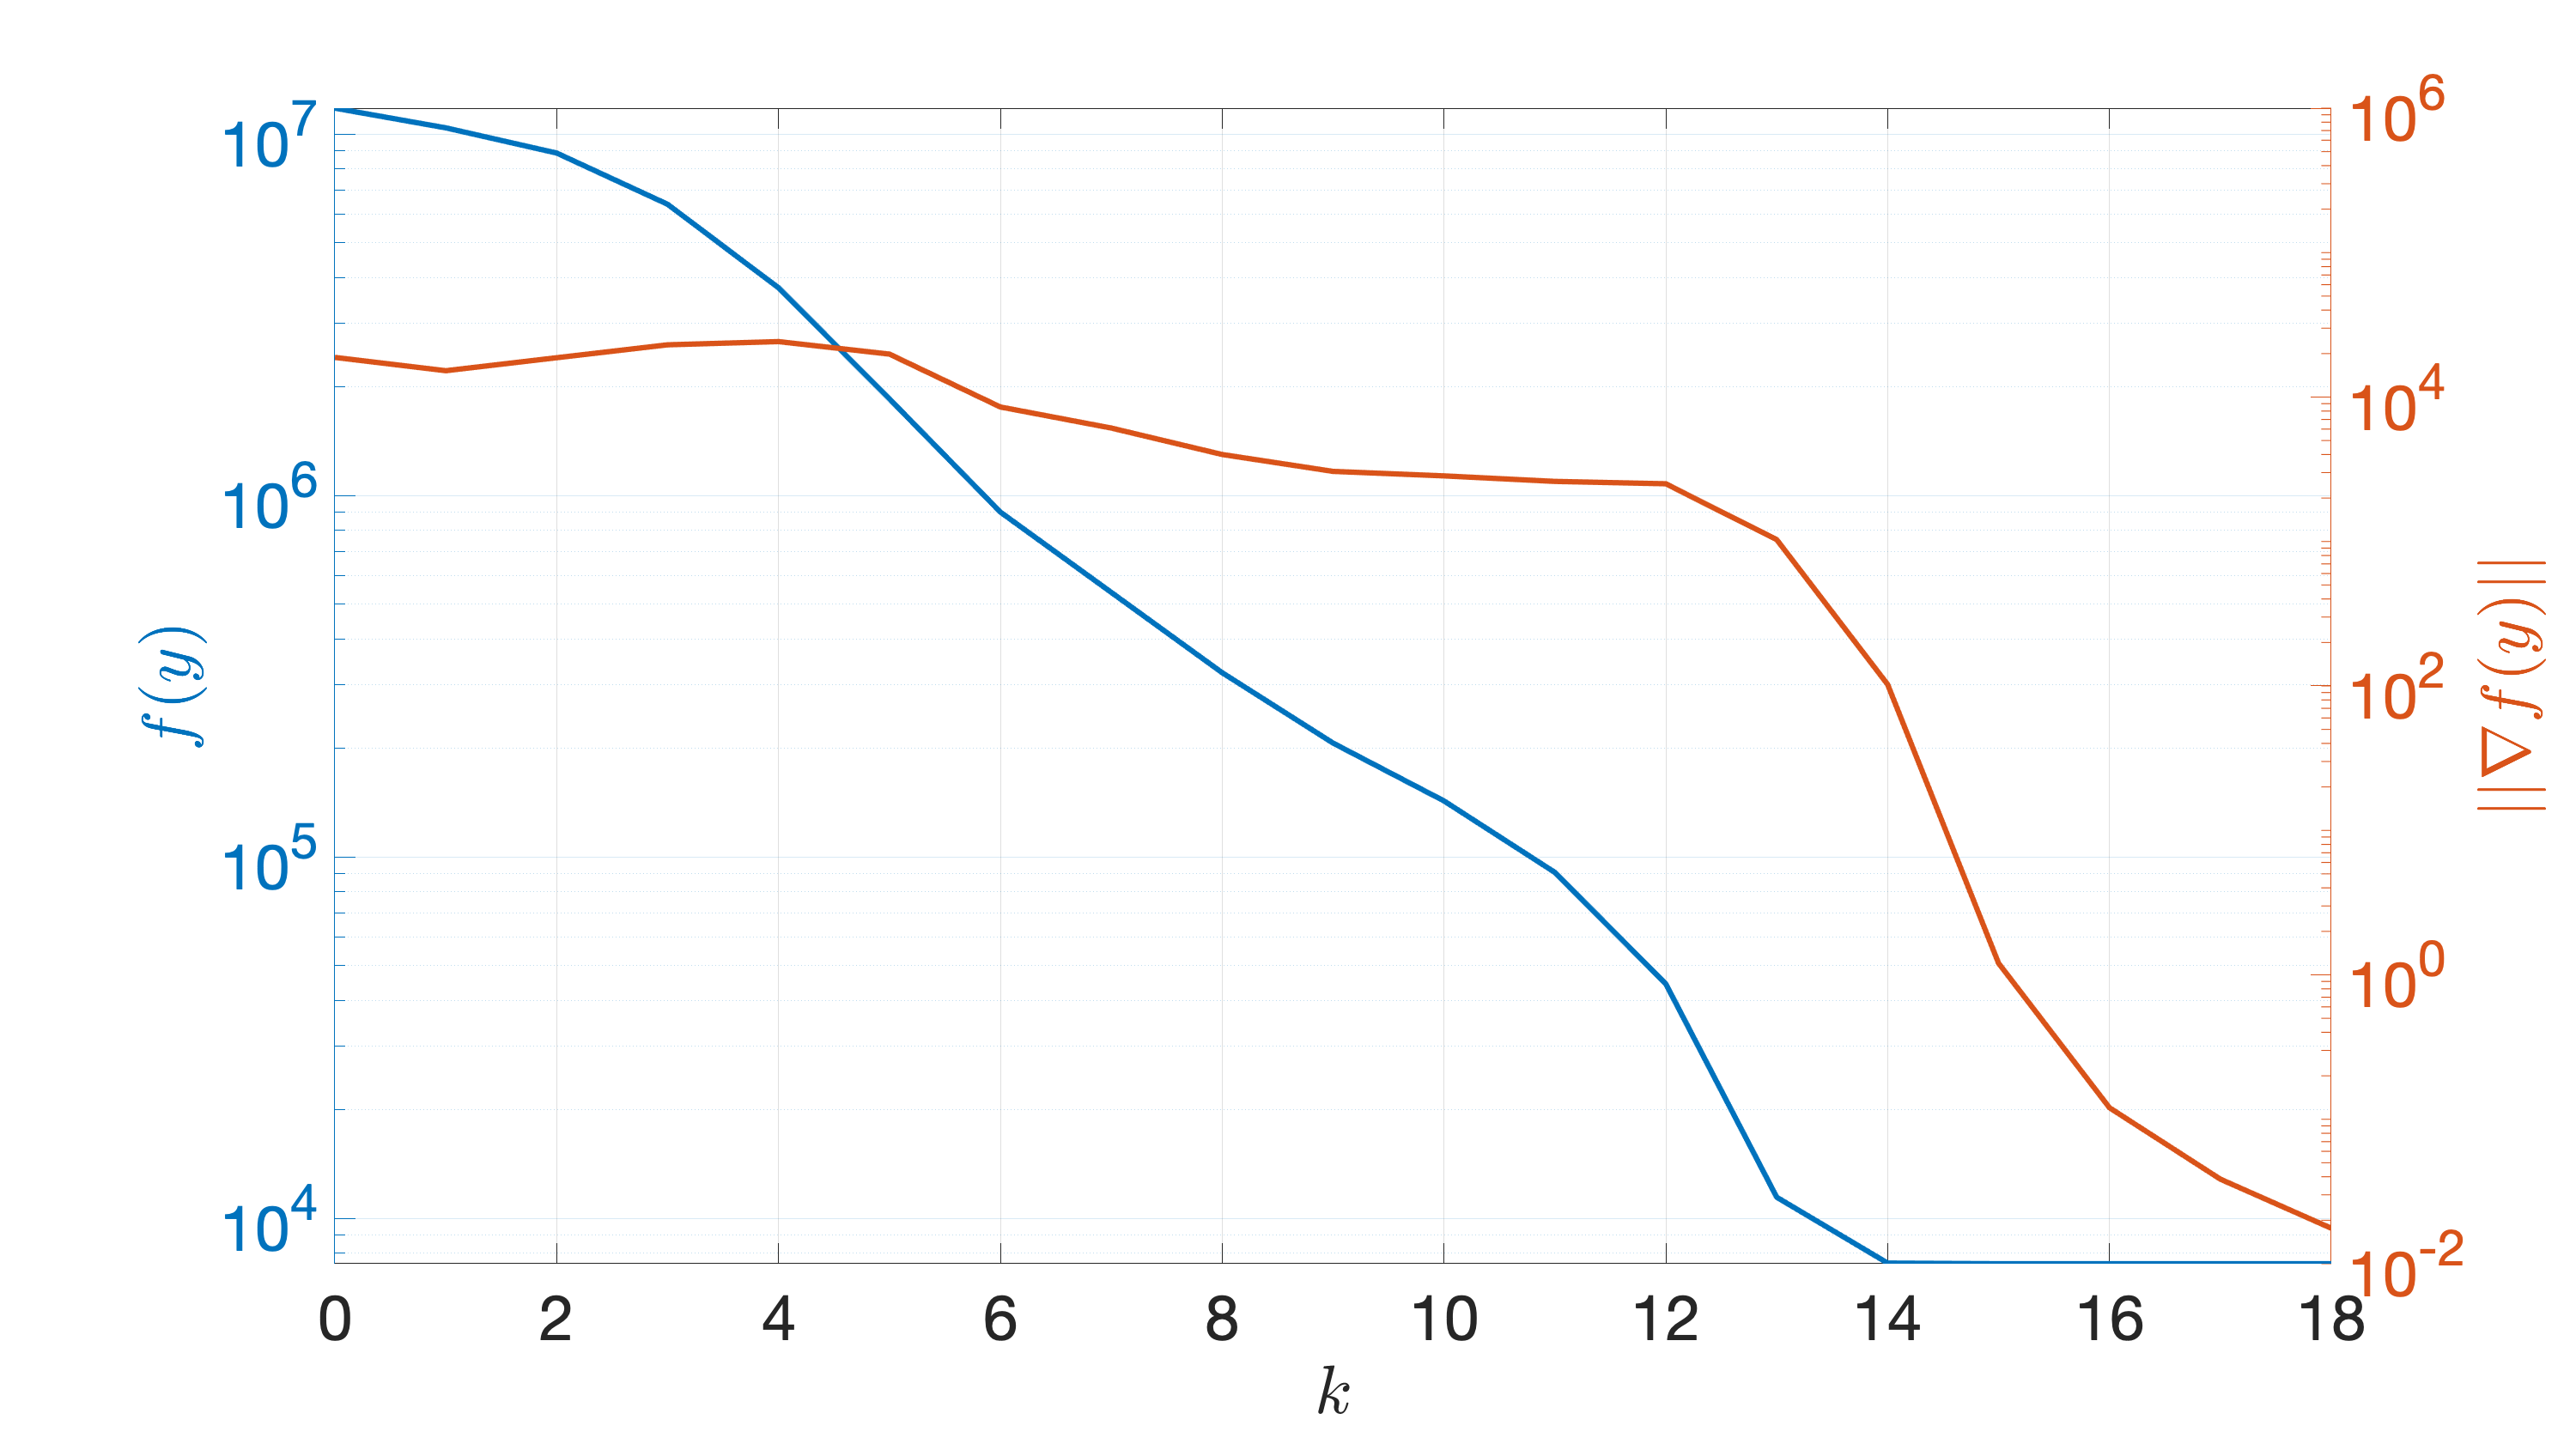
\includegraphics[width=0.9\textwidth]{figures/task3_LM_k_2.png}
			%\caption{Objective function value and gradient norm throughout the iterations of the LM algorithm for $k=2$.}
			\label{fig:task3_LM_k_2}
		\end{minipage}%
		\hfill
		\begin{minipage}[b]{0.5\textwidth}
			\centering
			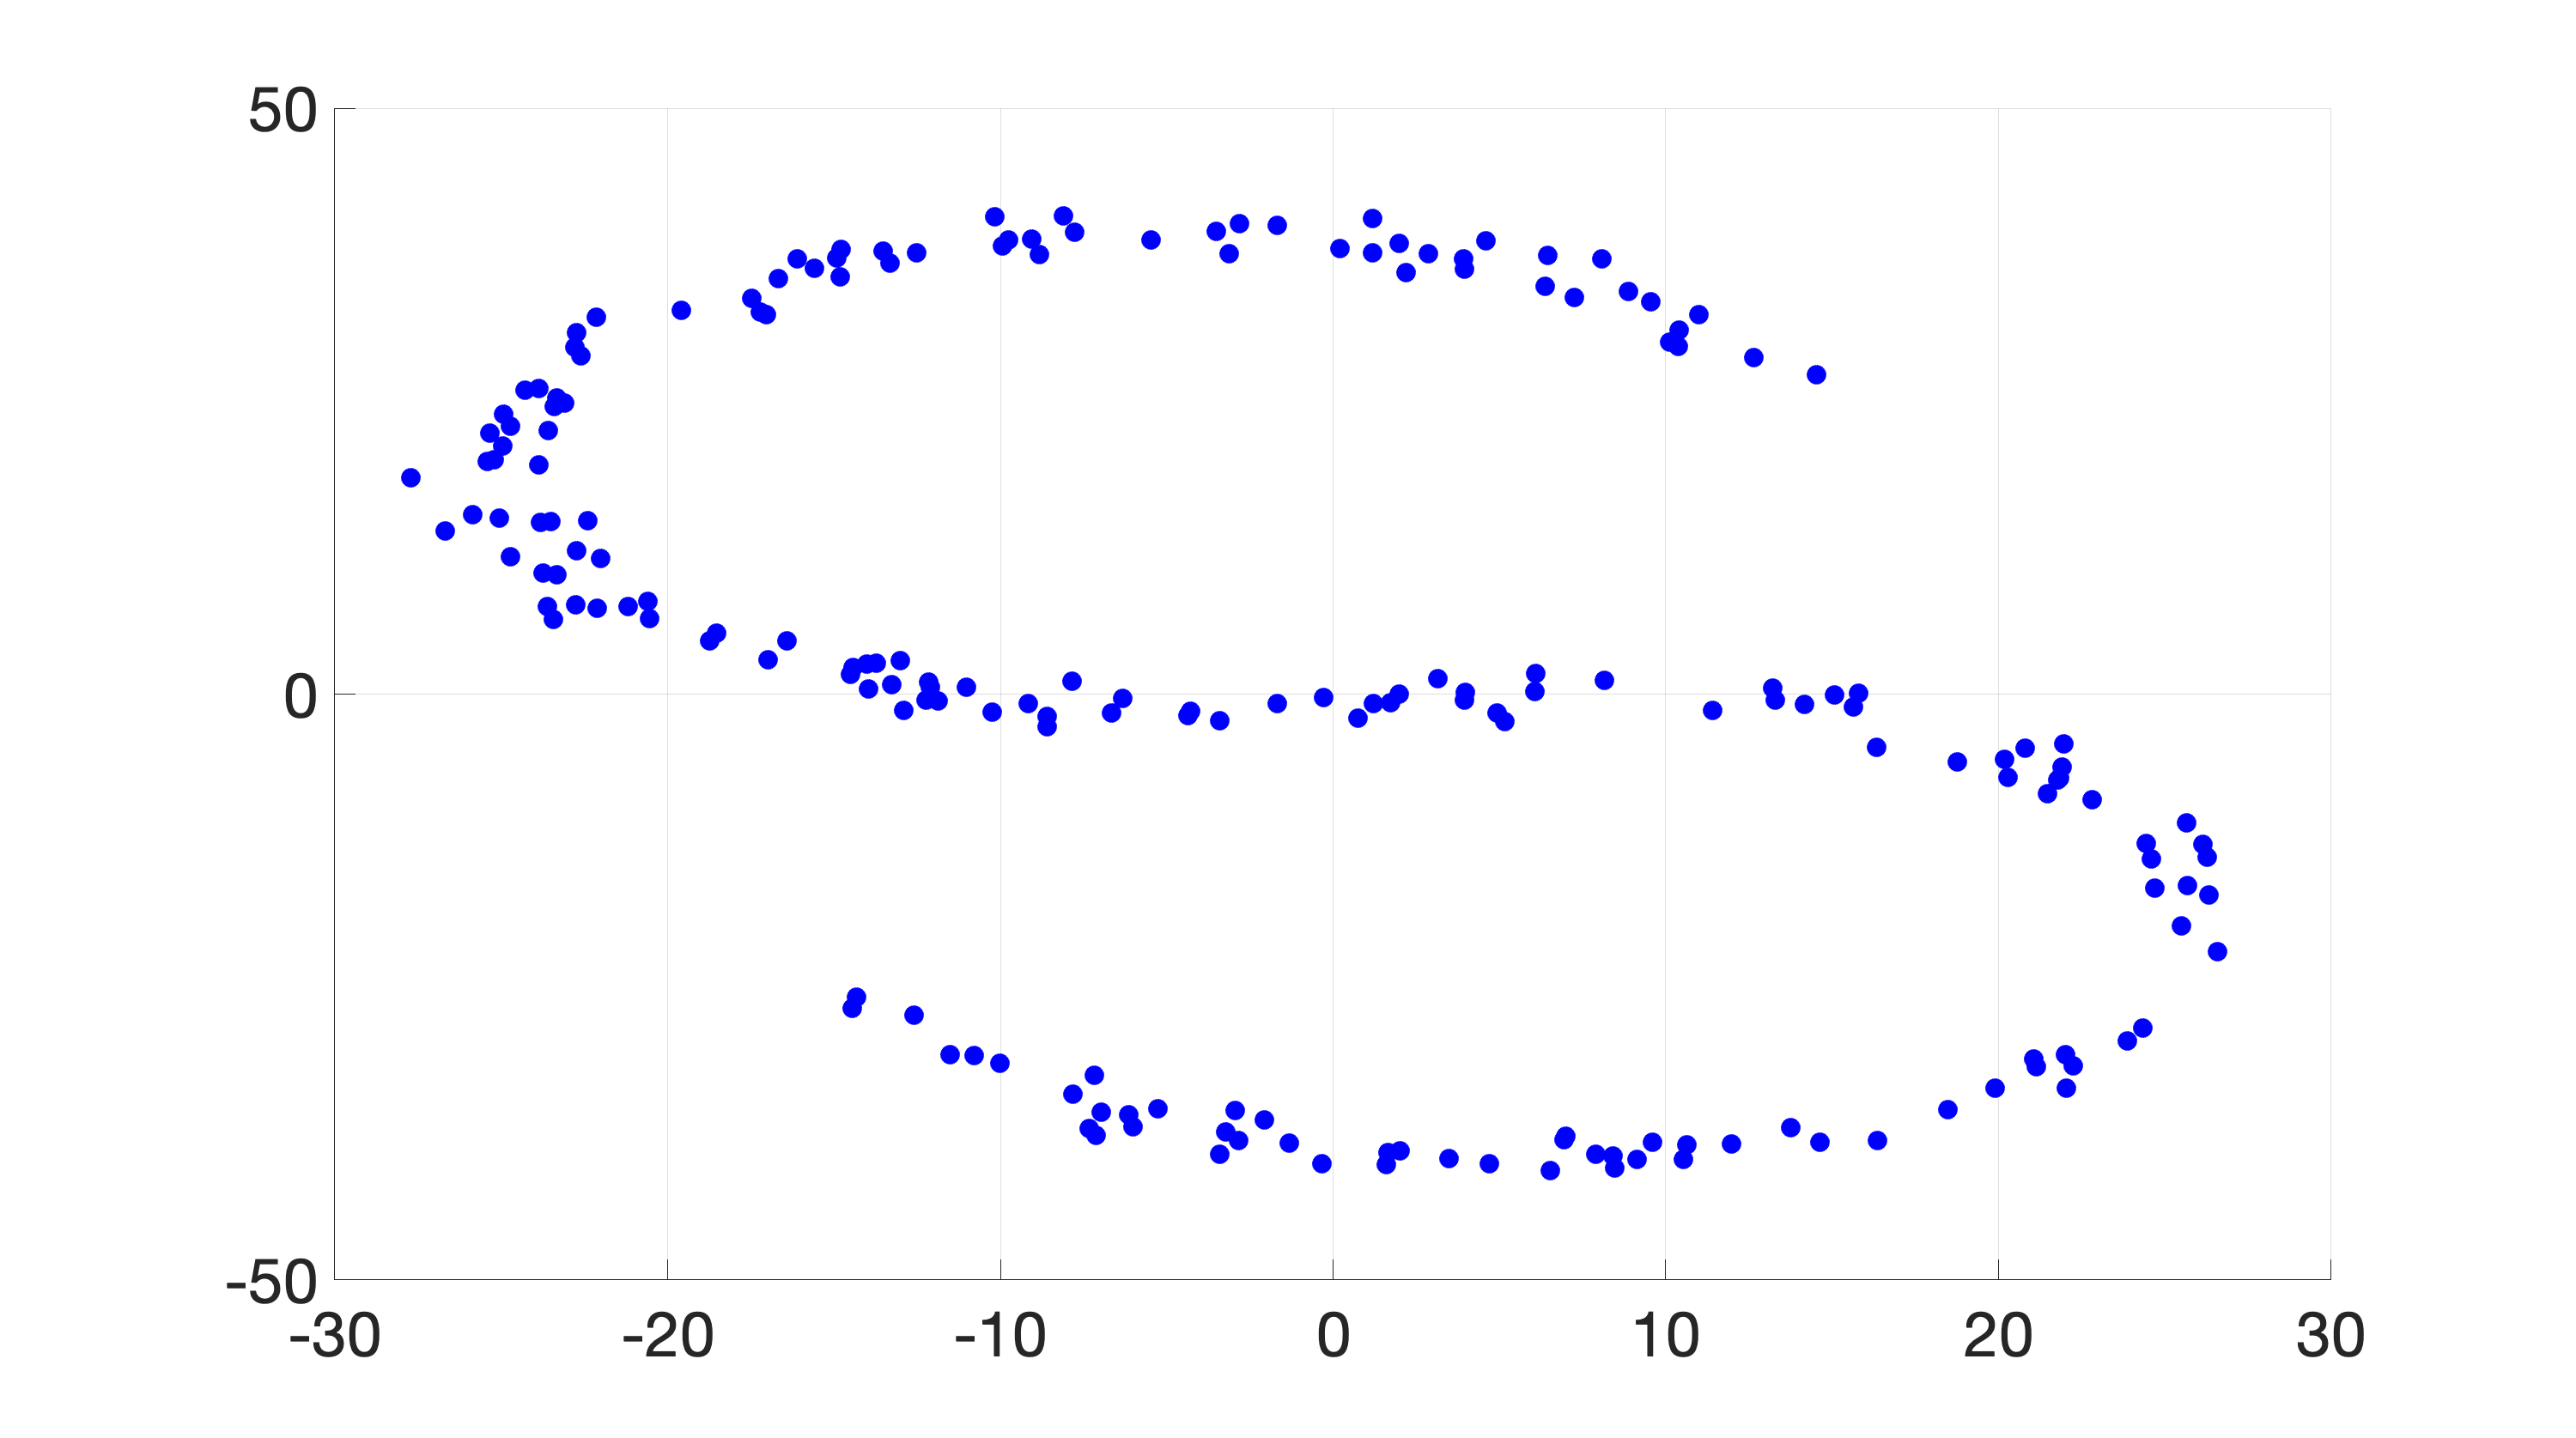
\includegraphics[width=0.9\textwidth]{figures/task3_lowerDim_k_2.png}
			%\caption{Solution to the optimization problem using the LM algorithm for $k=2$.}
			\label{fig:task3_lowerDim_k_2}
		\end{minipage}%
	\caption{$k=2$.}
	\end{figure}
\begin{figure}[ht]
	\centering
	\begin{minipage}[b]{0.5\textwidth}
		\centering
		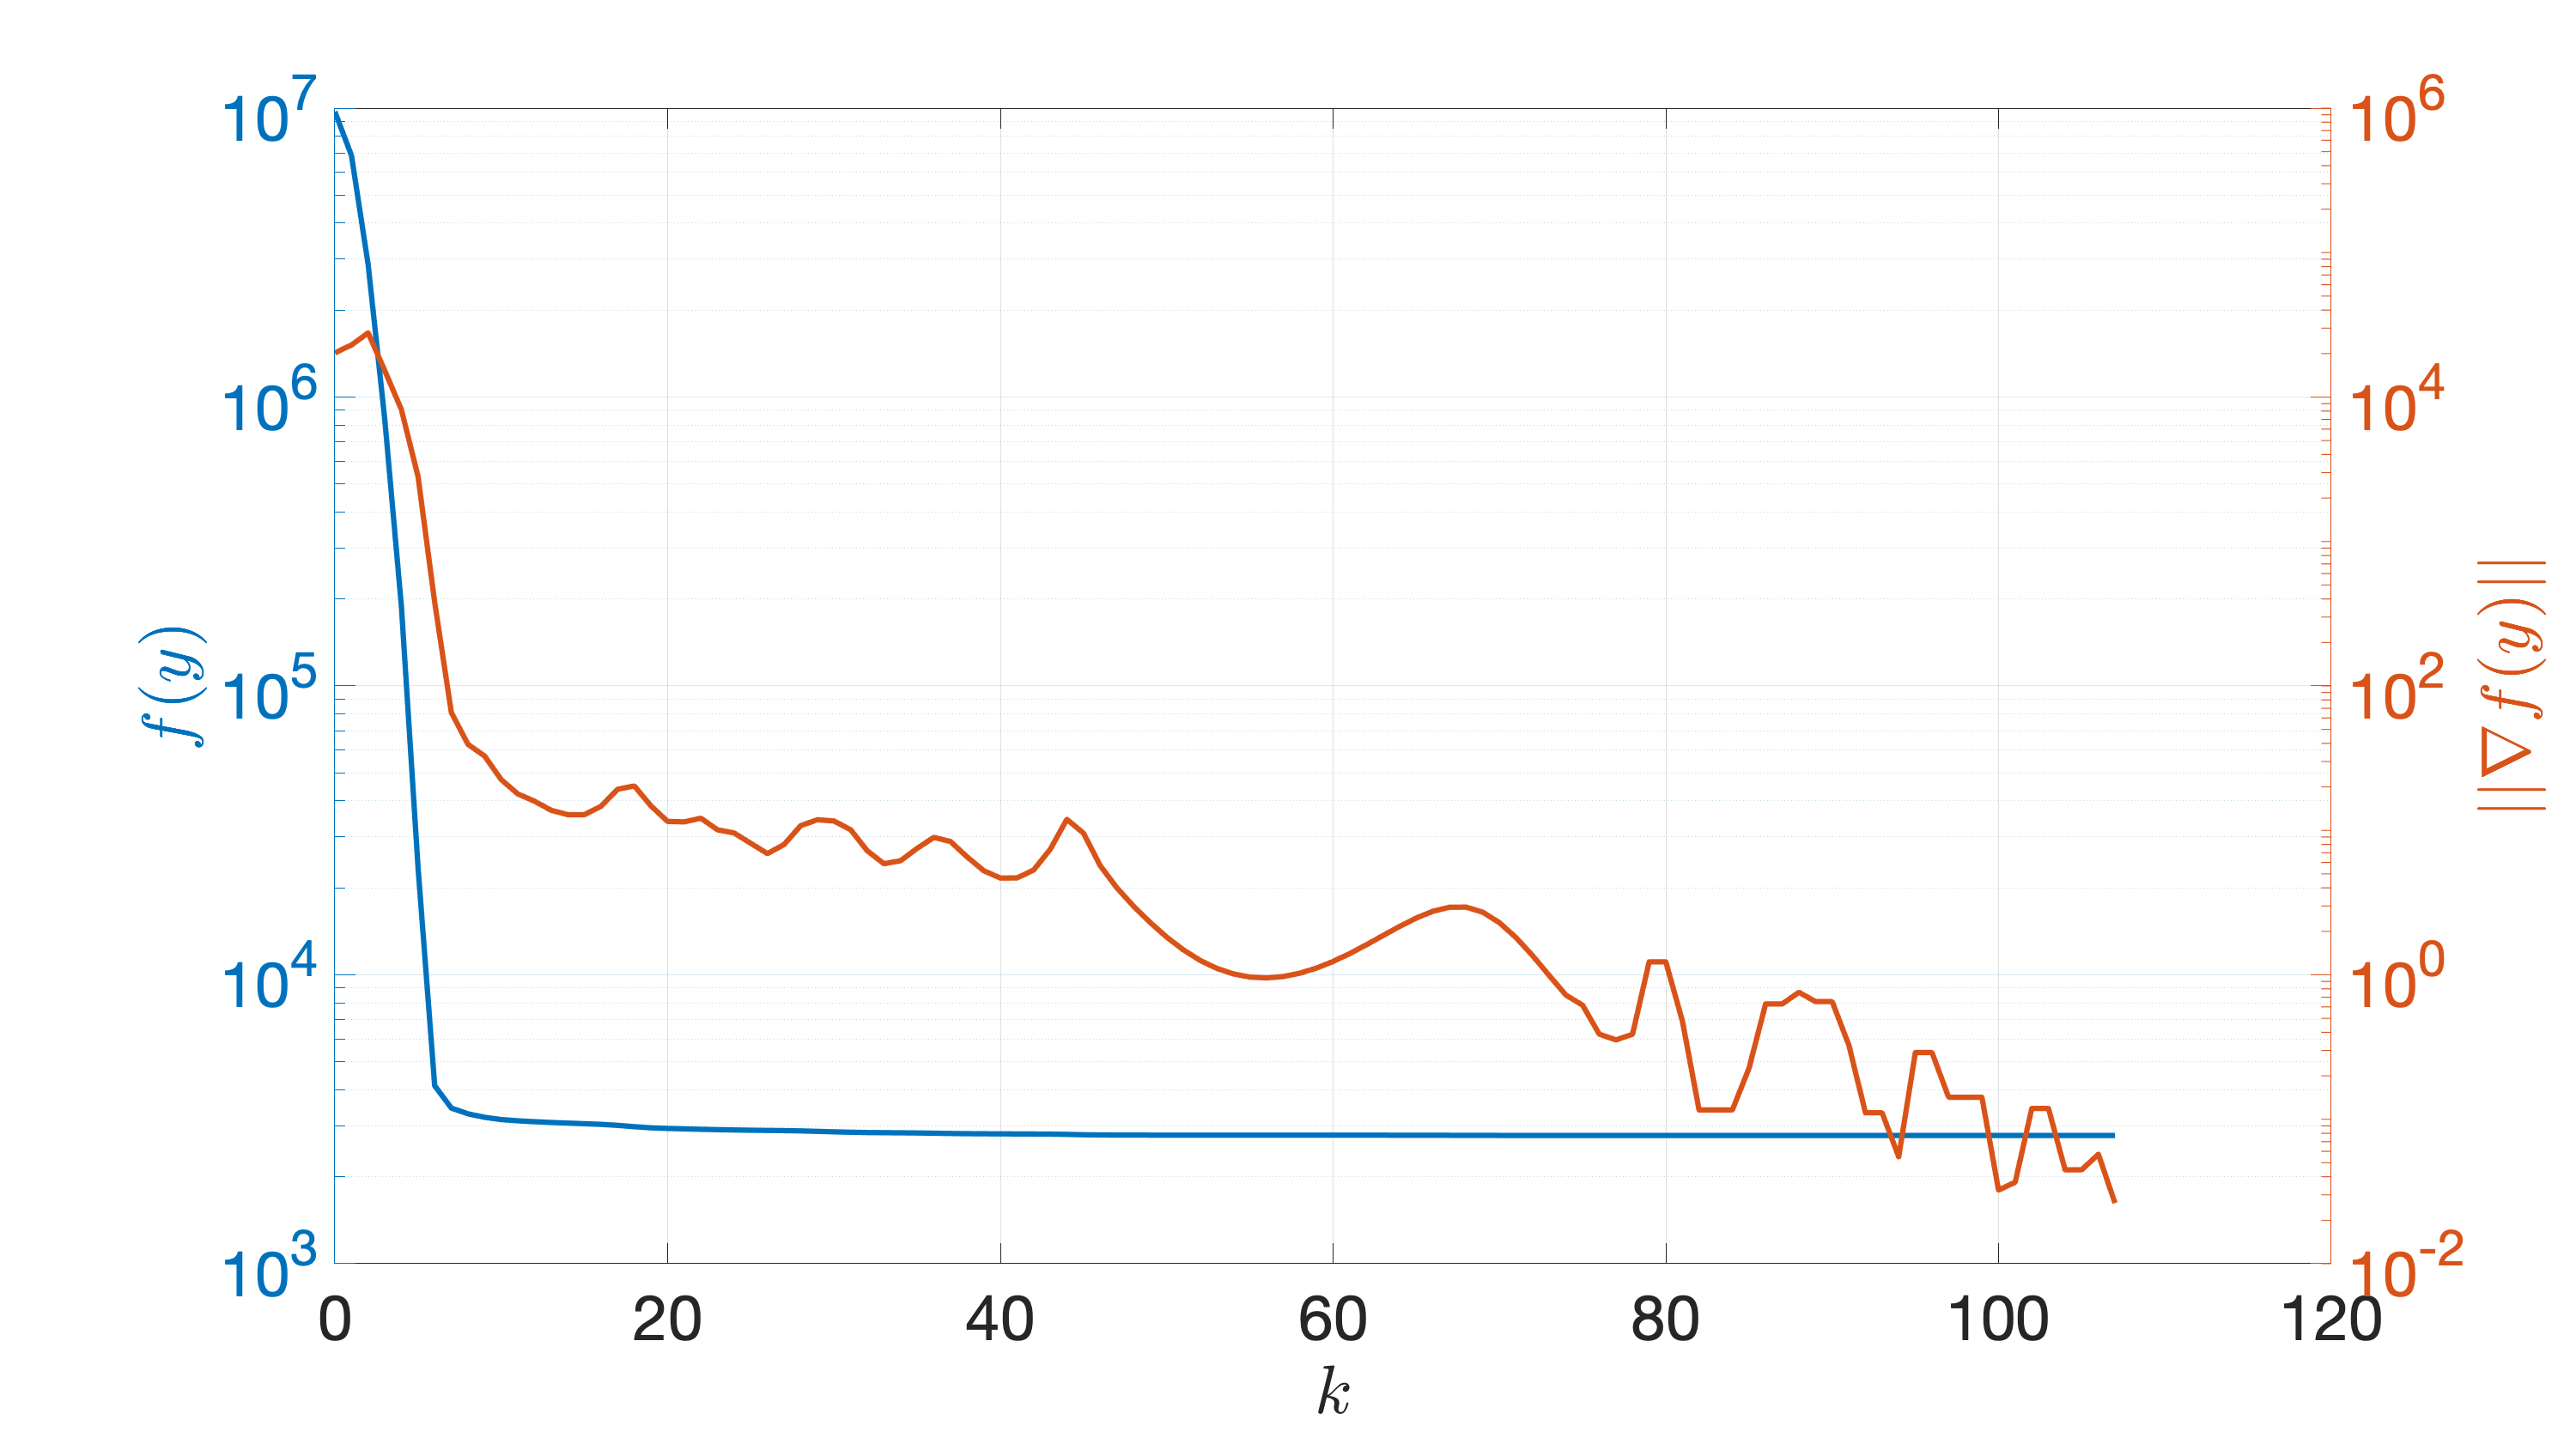
\includegraphics[width=0.9\textwidth]{figures/task3_LM_k_3.png}
		\label{fig:task3_LM_k_3}
	\end{minipage}%
	\hfill
	\begin{minipage}[b]{0.5\textwidth}
		\centering
	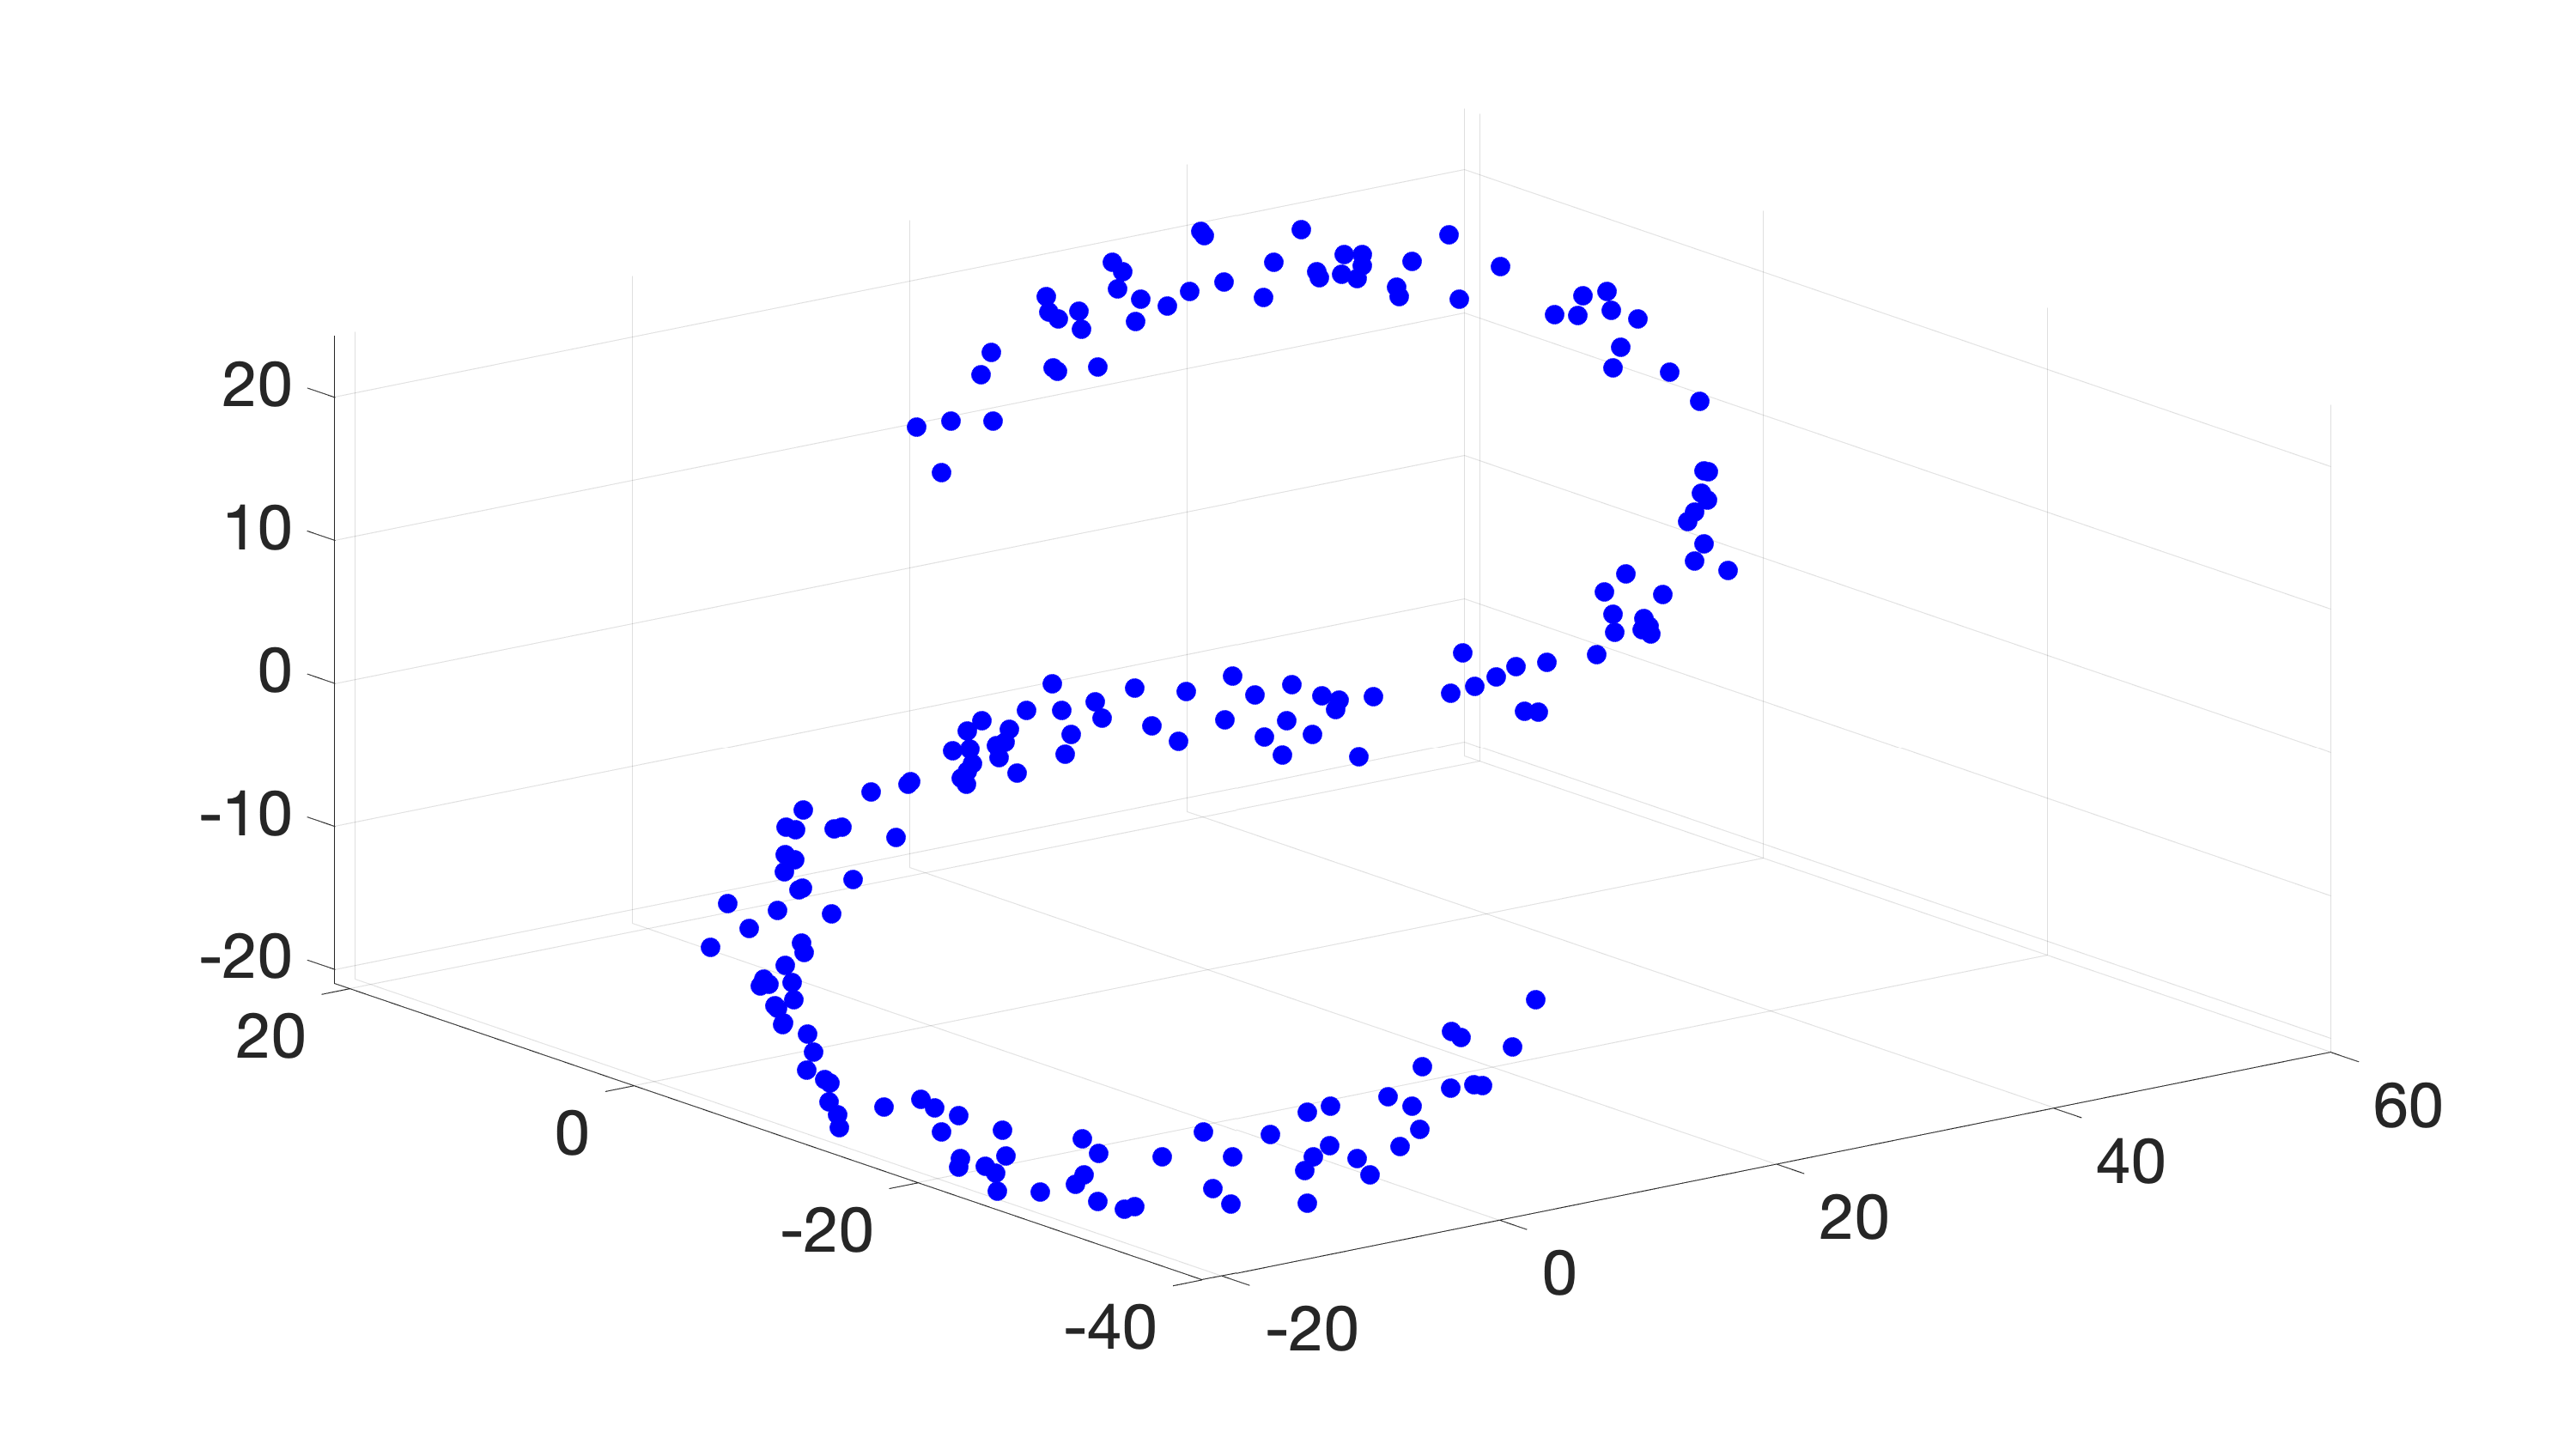
\includegraphics[width=0.9\textwidth]{figures/task3_lowerDim_k_3.png}
	\label{fig:task3_lowerDim_k_3}
	\end{minipage}%
\caption{$k=3$.}
\end{figure}
\end{comment}

\end{frame}

\begin{frame}{Part 3 - Task 4}
	Não é dada inicialização:
	\begin{itemize}
		\item Resolver o problema com LM para vários $\mathbf{y}_0$ aleatórios
		\item Cada LM pode ser calculado em paralelo
		\item Escolhe-se a melhor solução 
	\end{itemize}
\begin{figure}[ht]
	\centering
	\begin{minipage}[b]{0.5\textwidth}
		\centering
		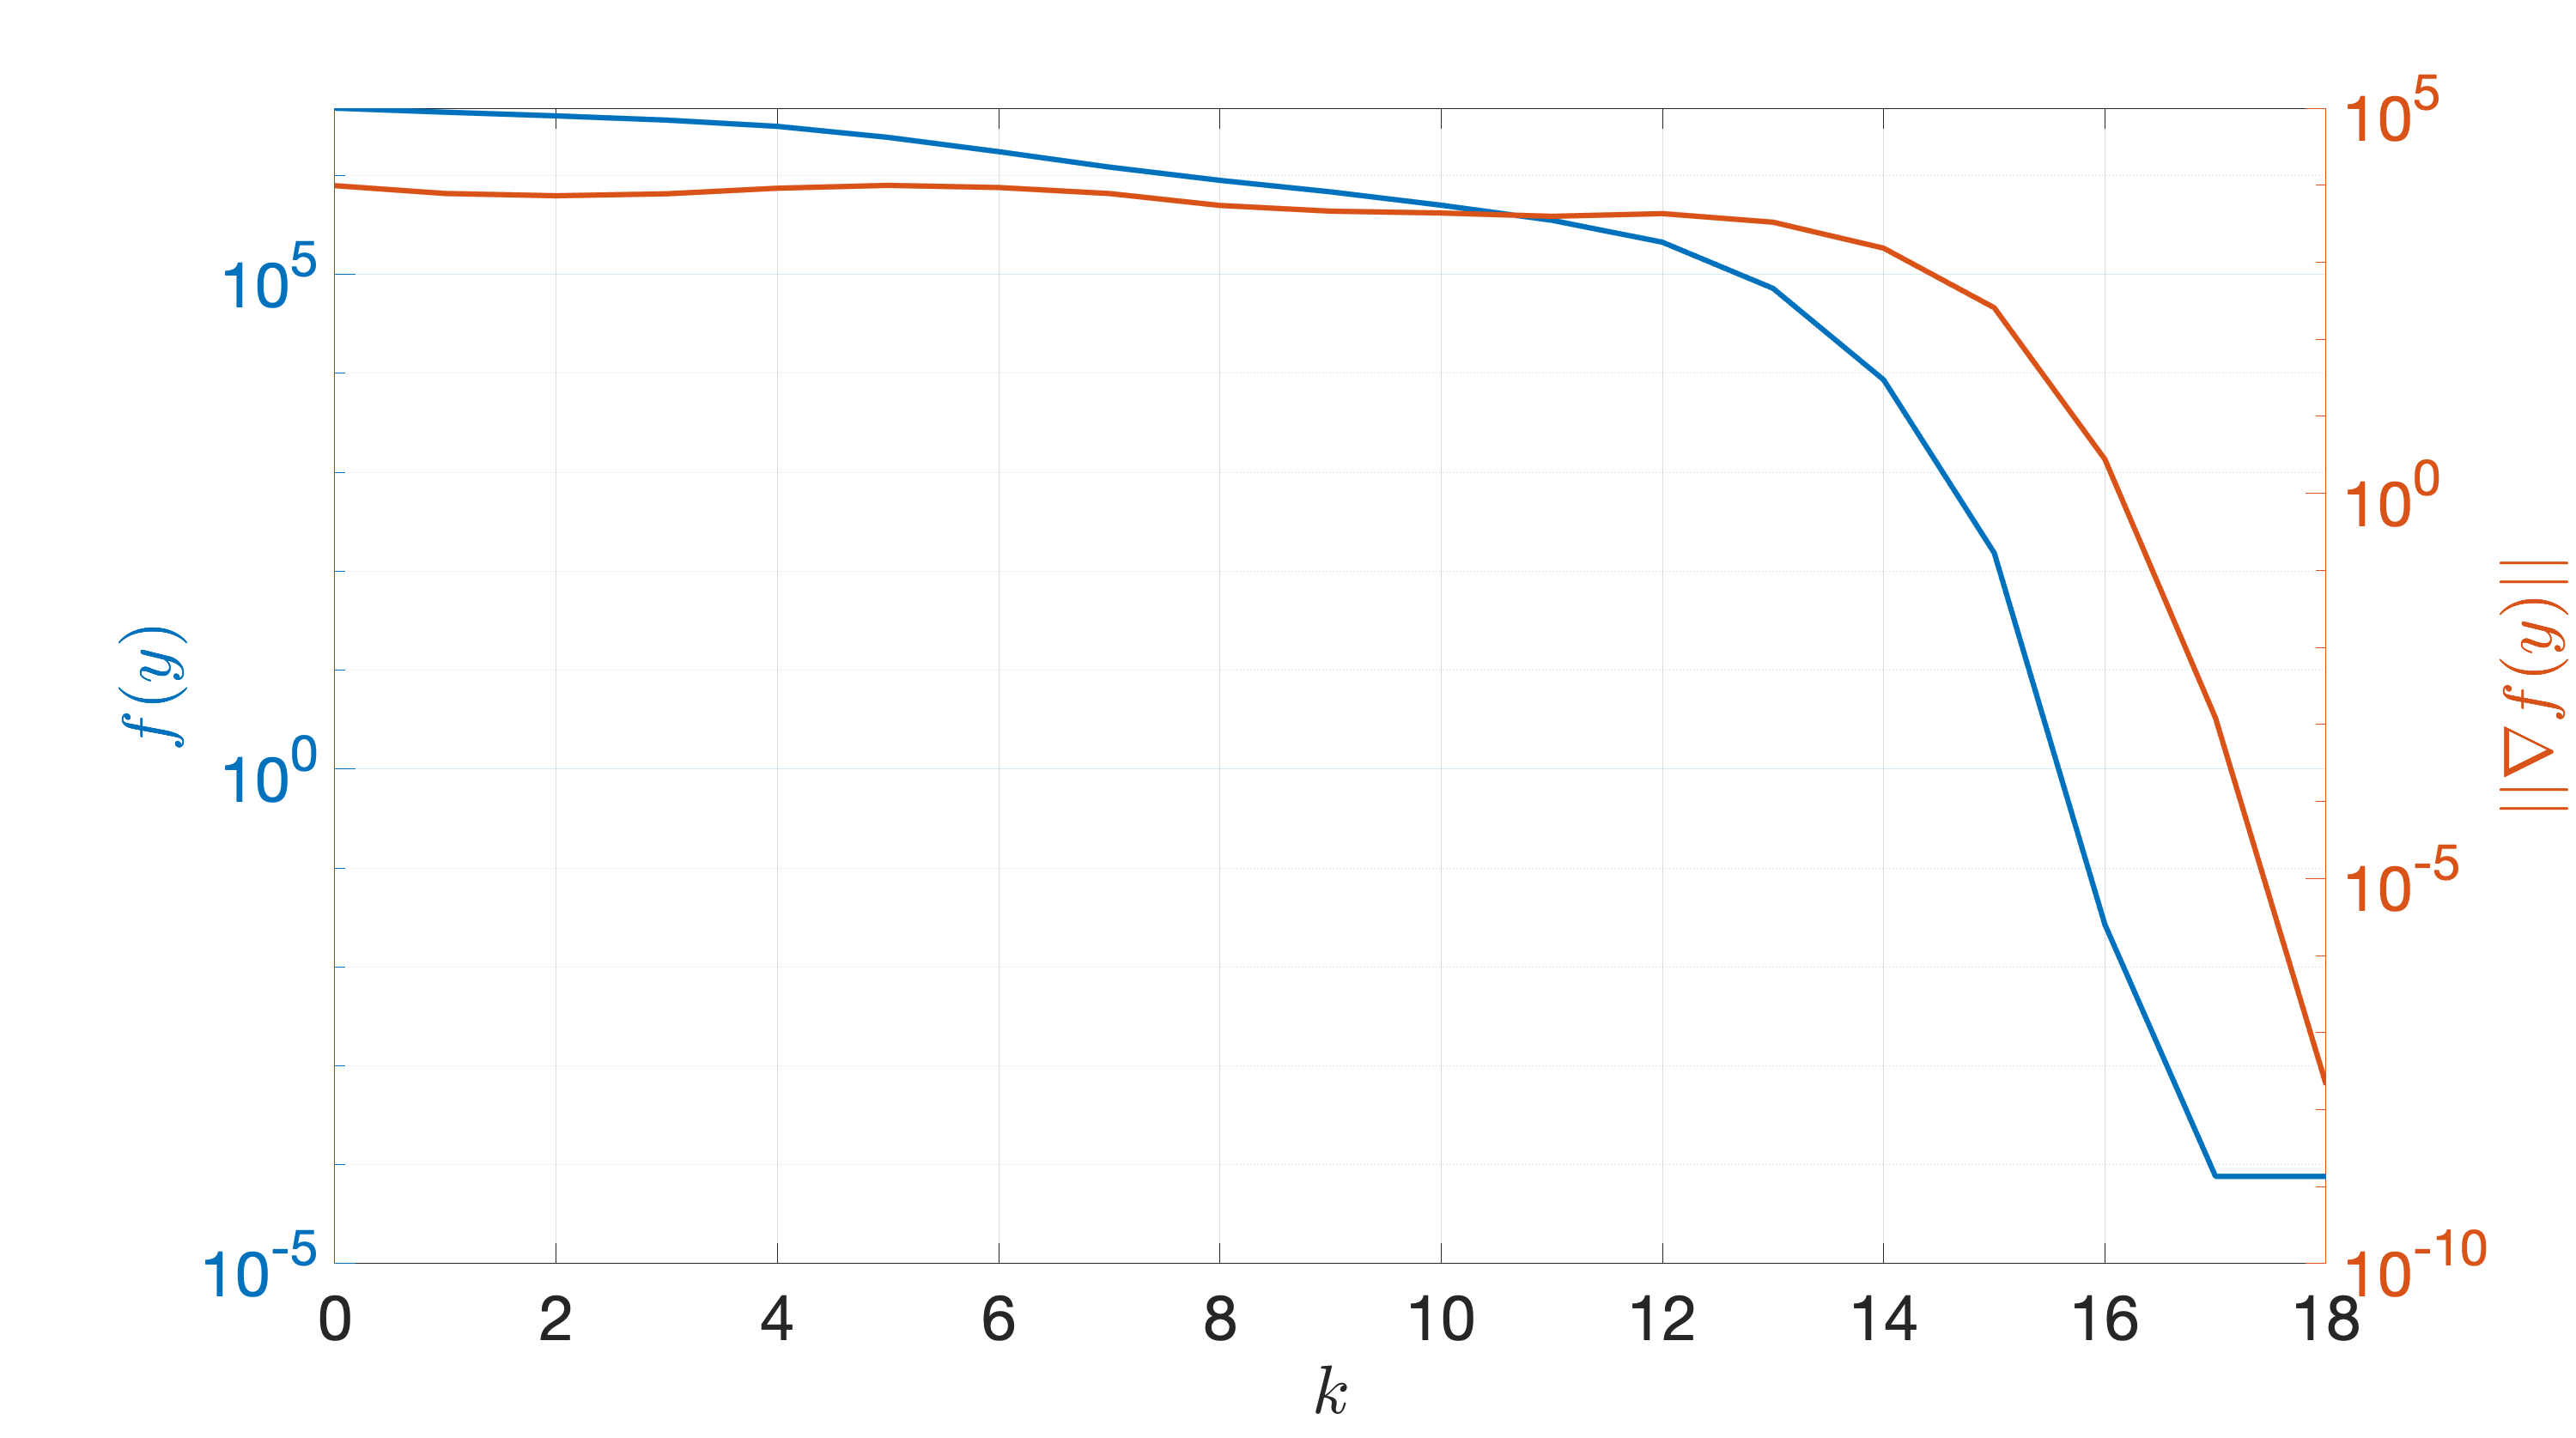
\includegraphics[width=0.9\textwidth]{figures/task4_LM.png}
		\label{fig:task4_LM}
	\end{minipage}%
	\hfill
	\begin{minipage}[b]{0.5\textwidth}
		\centering
		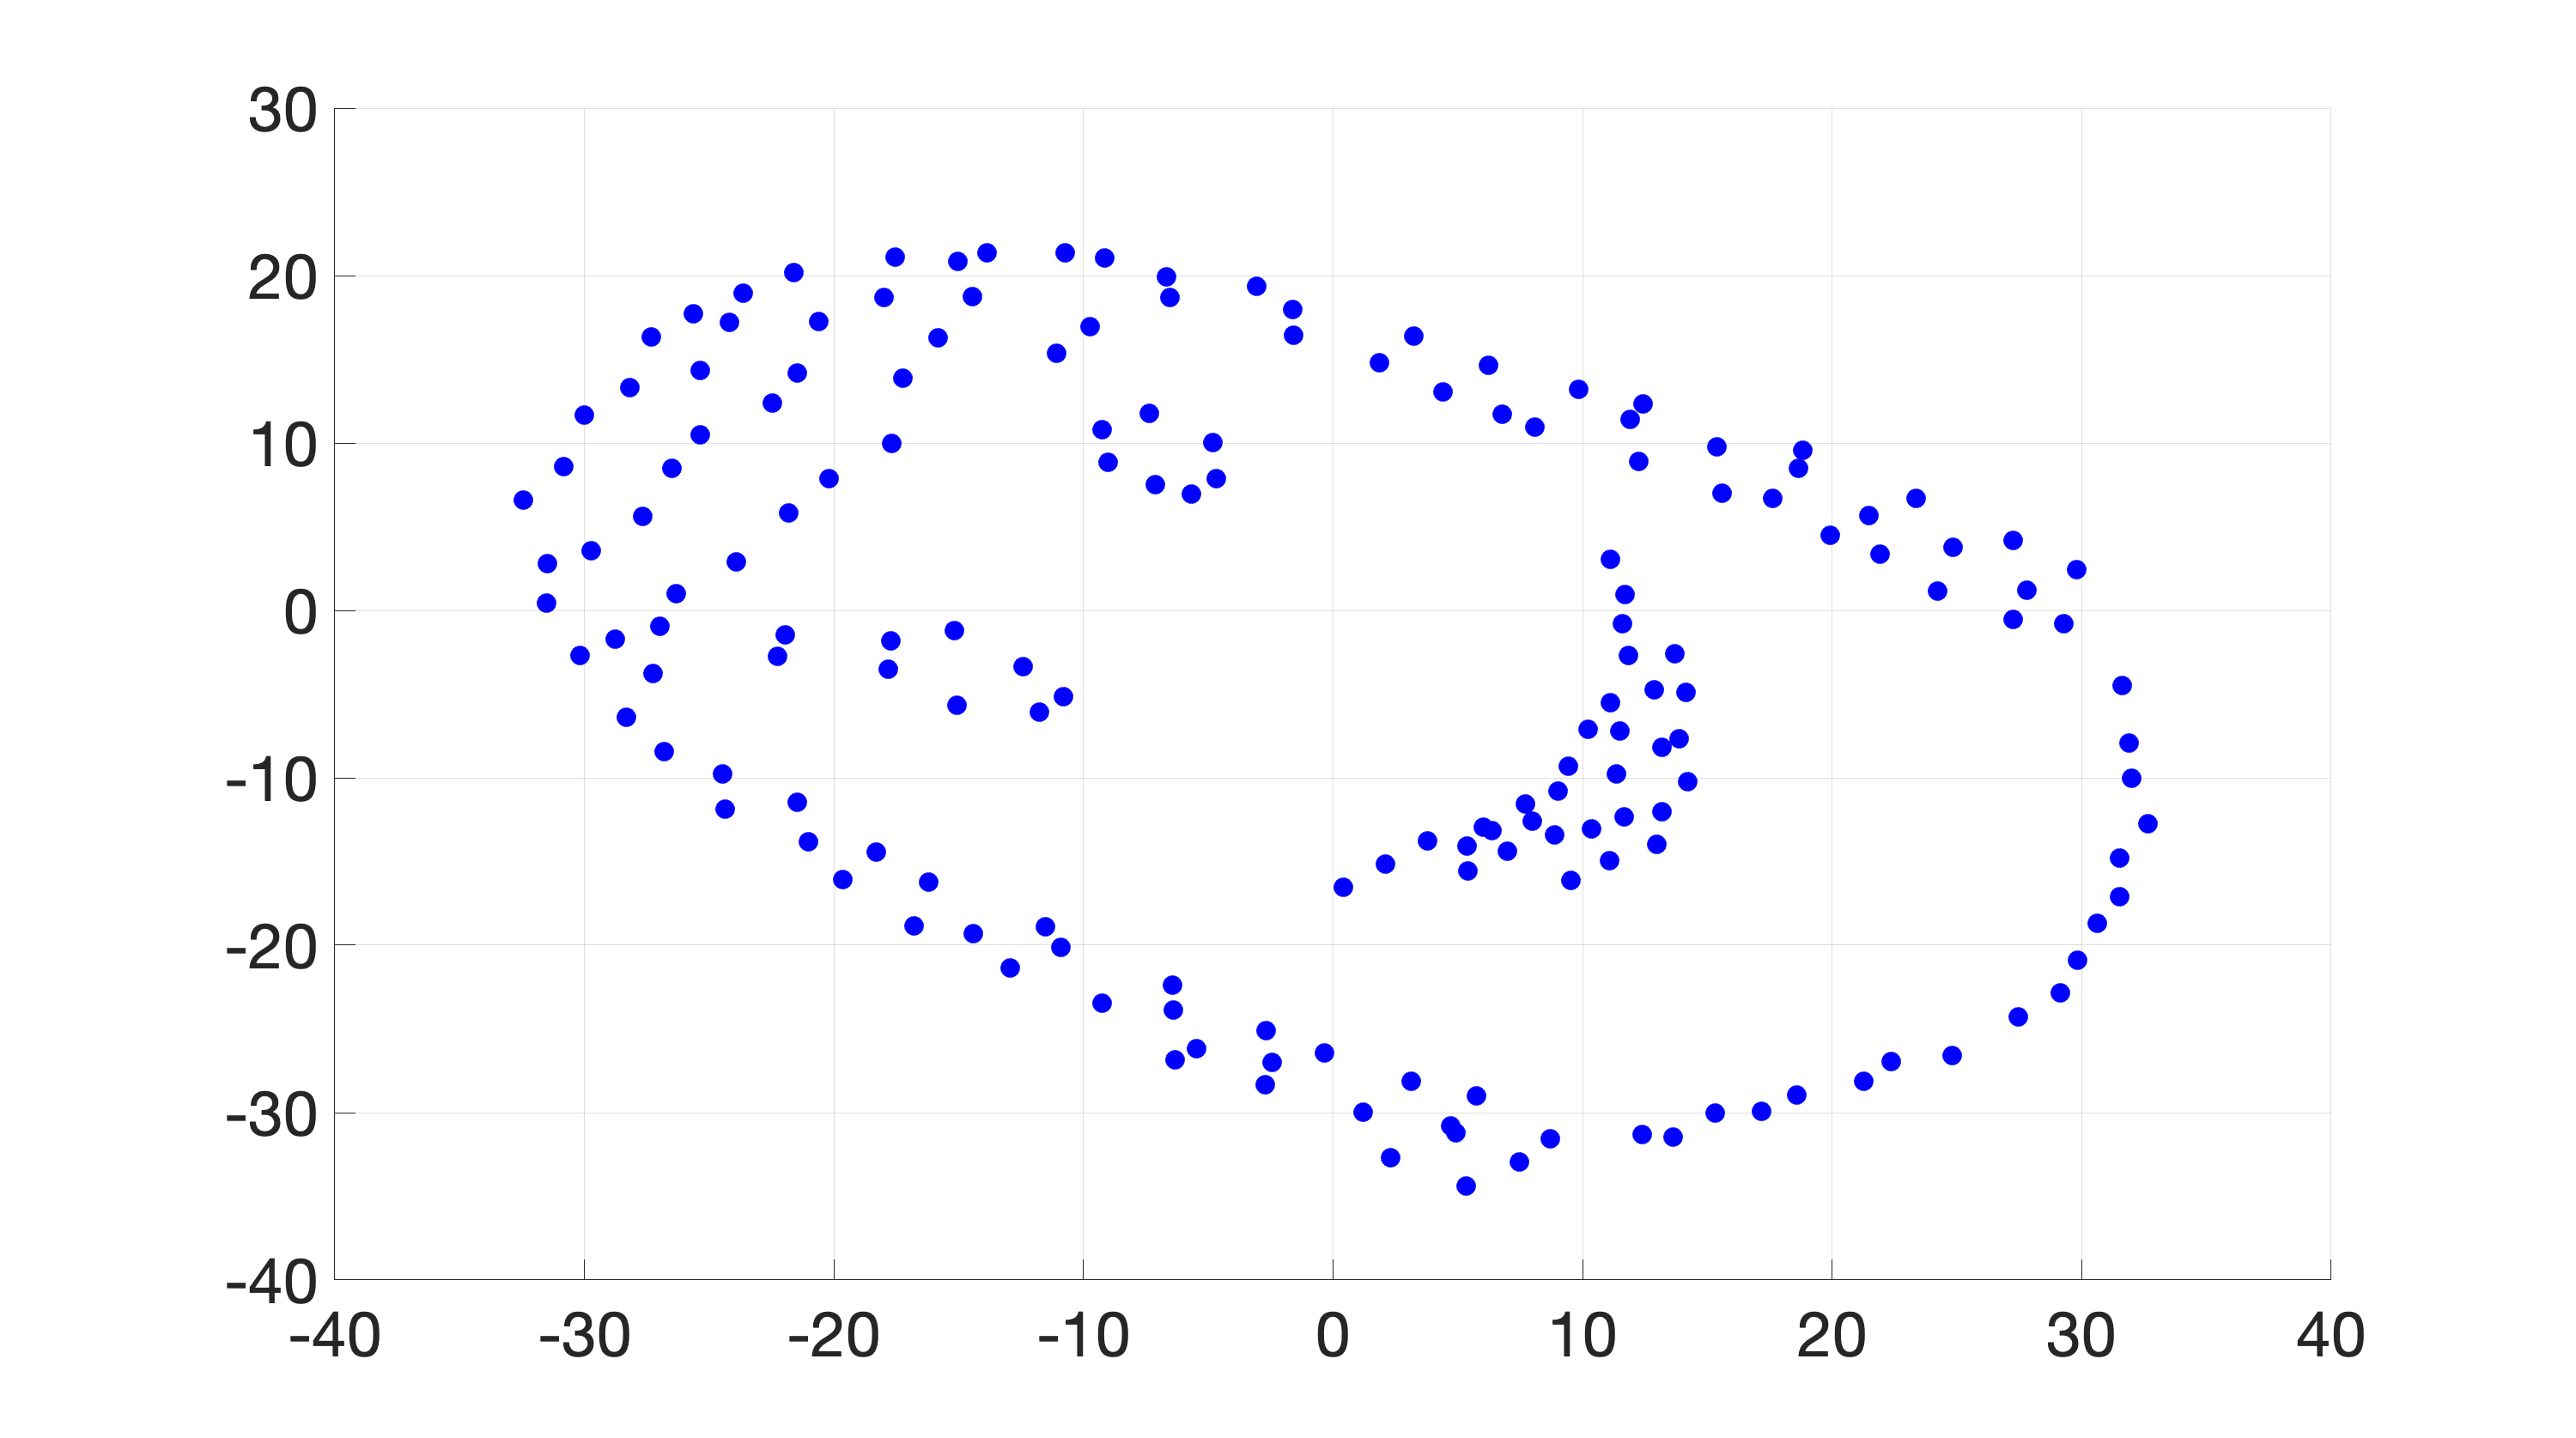
\includegraphics[width=0.9\textwidth]{figures/task4_sol.png}
		\label{fig:task4_sol}
	\end{minipage}%
	\caption{Melhor solução em 24 inicializações distintas para $k=2$.}
\end{figure}
	 
\end{frame}

\begin{frame}{Part 3 - Task 4}
	Verificou-se que:
	\begin{itemize}
		\item Para todas as 24 inicializações obtém-se o mesmo valor de $f$
		\item As verificam $f(\mathbf{y}_{sol}) = 7.6430\times 10^{-5}$
		\item A função de otimização é não-negativa
		\item Se se reduzir $\epsilon$, $f(\mathbf{y}_{sol})$ aproxima-se de 0
		\item Na prática, pode ser considerado um mínimo global ($f(\mathbf{y}_{sol})<< D_{ij}$)
		\end{itemize}
\end{frame}

\begin{frame}{Part 3 - Task 4 - Unicidade da solução}
	Seja
	\begin{equation*}\label{key}
	\bar{\mathbf{y}} = \mathrm{col}(\mathcal{T}\mathbf{y_1}+\mathbf{w},\ldots,\mathcal{T}\mathbf{y_N}+\mathbf{w})\:,
	\end{equation*}
onde $\mathcal{T} \in \mathbb{R}^{k\times k}$ é uma matriz de rotação e $\mathbf{w}\in\mathbb{R}^{k}$. É evidente que
	\begin{equation*}\label{key}
	||\mathbf{\bar{y}_m}-{\mathbf{\bar{y}_n}}|| = ||\mathbf{y_m}-\mathbf{y_n}||
	\end{equation*}
	para qualquer par $(m,n):m \in \{1,\ldots,N\}, n \in \{1,\ldots,N\}$. Logo
	\begin{equation*}\label{key}
	f(\mathbf{\bar{y}}) = f(\mathbf{y})\:.
	\end{equation*}
	\begin{itemize}
		\item Se for encontrada uma solução, então existe uma infinidade de soluções.
		\item Logo, a solução encontrada não é única.
	\end{itemize}
\end{frame}

\begin{frame}{Part 3 - Task 4 - Unicidade da solução}
\begin{figure}[ht]
	\centering
	\begin{minipage}[b]{0.5\textwidth}
		\centering
		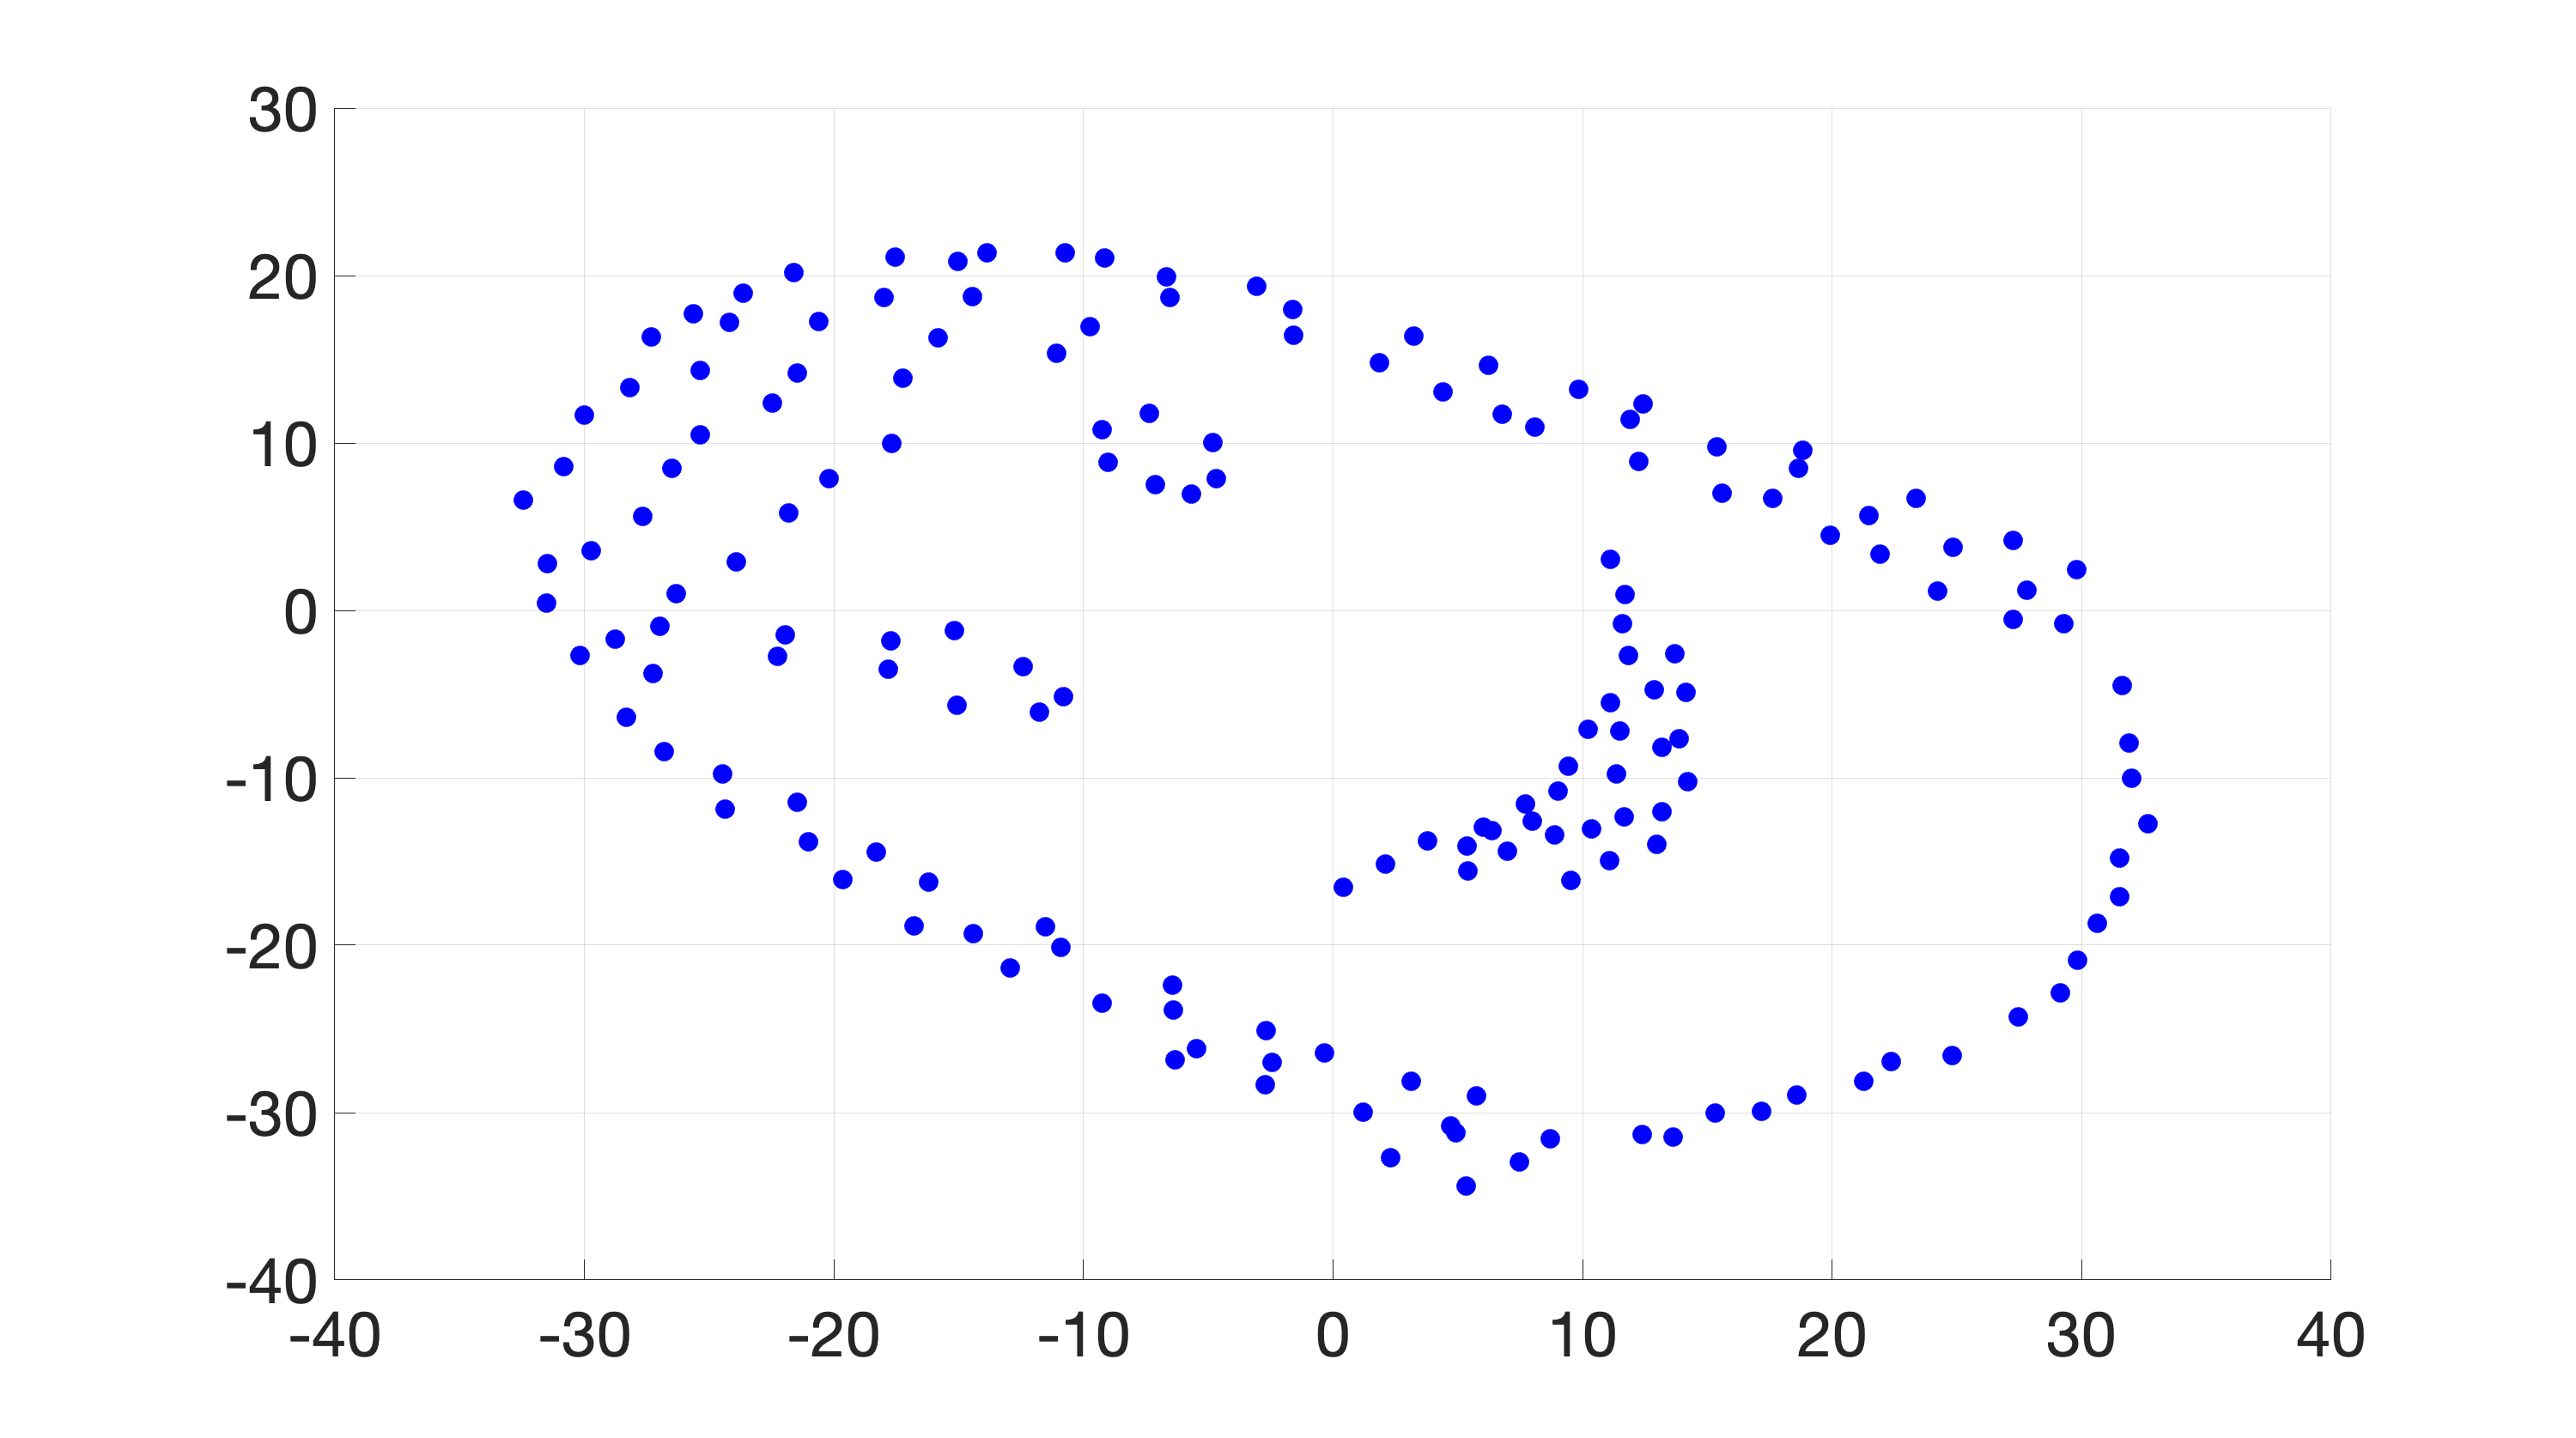
\includegraphics[width=0.9\textwidth]{figures/task4_sol.png}
		\label{fig:task4_LM}
	\end{minipage}%
	\hfill
	\begin{minipage}[b]{0.5\textwidth}
		\centering
		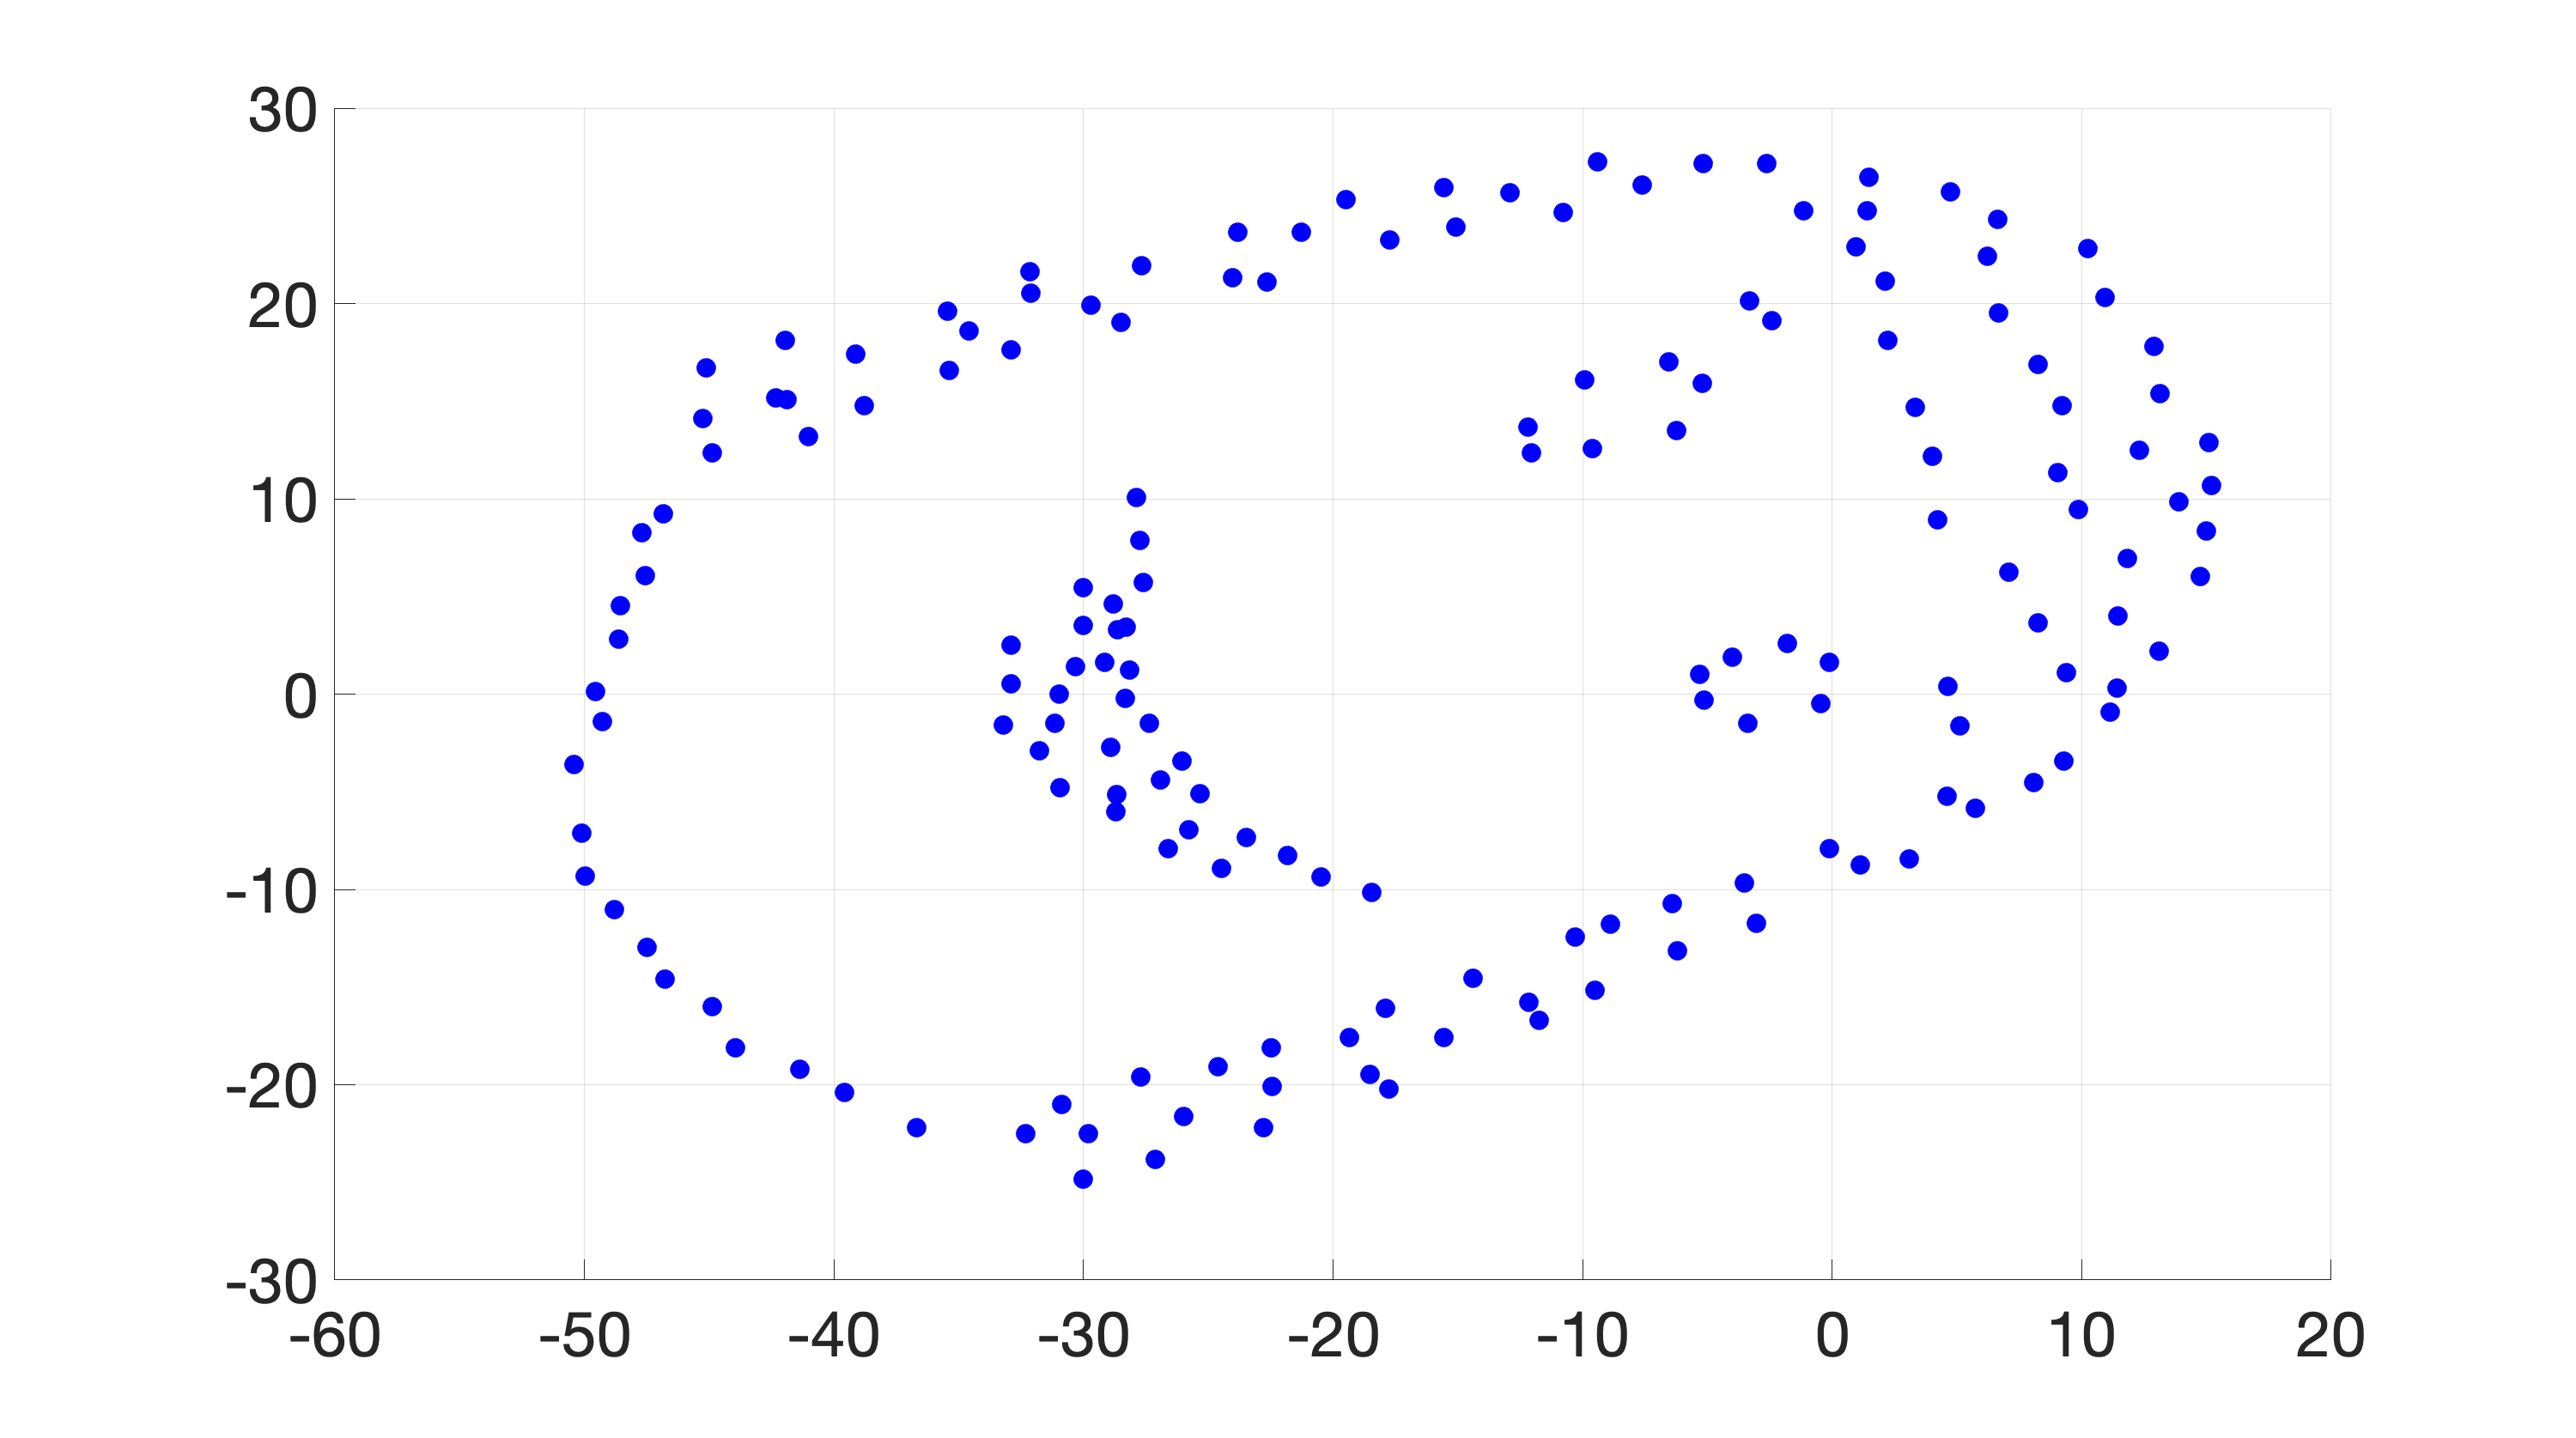
\includegraphics[width=0.9\textwidth]{figures/task4_sol_2.png}
		\label{fig:task4_sol}
	\end{minipage}%
	\caption{Duas melhores soluções em 24 inicializações distintas para $k=2$.}
\end{figure}
\begin{itemize}
	\item Uma solução pode ser obtida da outra por via de uma rotação e translação de cada $\mathbf{y_i}, \; i \in \{1,\ldots,N\}$.
\end{itemize}
\end{frame}

\begin{frame}{Part 3 - Task 4 - Unicidade da solução}
	\begin{itemize}
		\item Será que todas as soluções são da forma 
		\begin{equation*}\label{key}
		\bar{\mathbf{y}} = \mathrm{col}(\mathcal{T}\mathbf{y_1}+\mathbf{w},\ldots,\mathcal{T}\mathbf{y_N}+\mathbf{w})\:?
		\end{equation*}
	\end{itemize}
	\begin{itemize}
	\item Não! A reflexão de cada $\mathbf{y_i}, \; i \in \{1,\ldots,N\}$ em relação ao eixo da primeira coordenada origina um valor igual da função de custo.
\end{itemize}
\end{frame}


\begin{frame}{Part 3 - Task 4 - cMDS}
	\begin{figure}[ht]
		
			\centering
			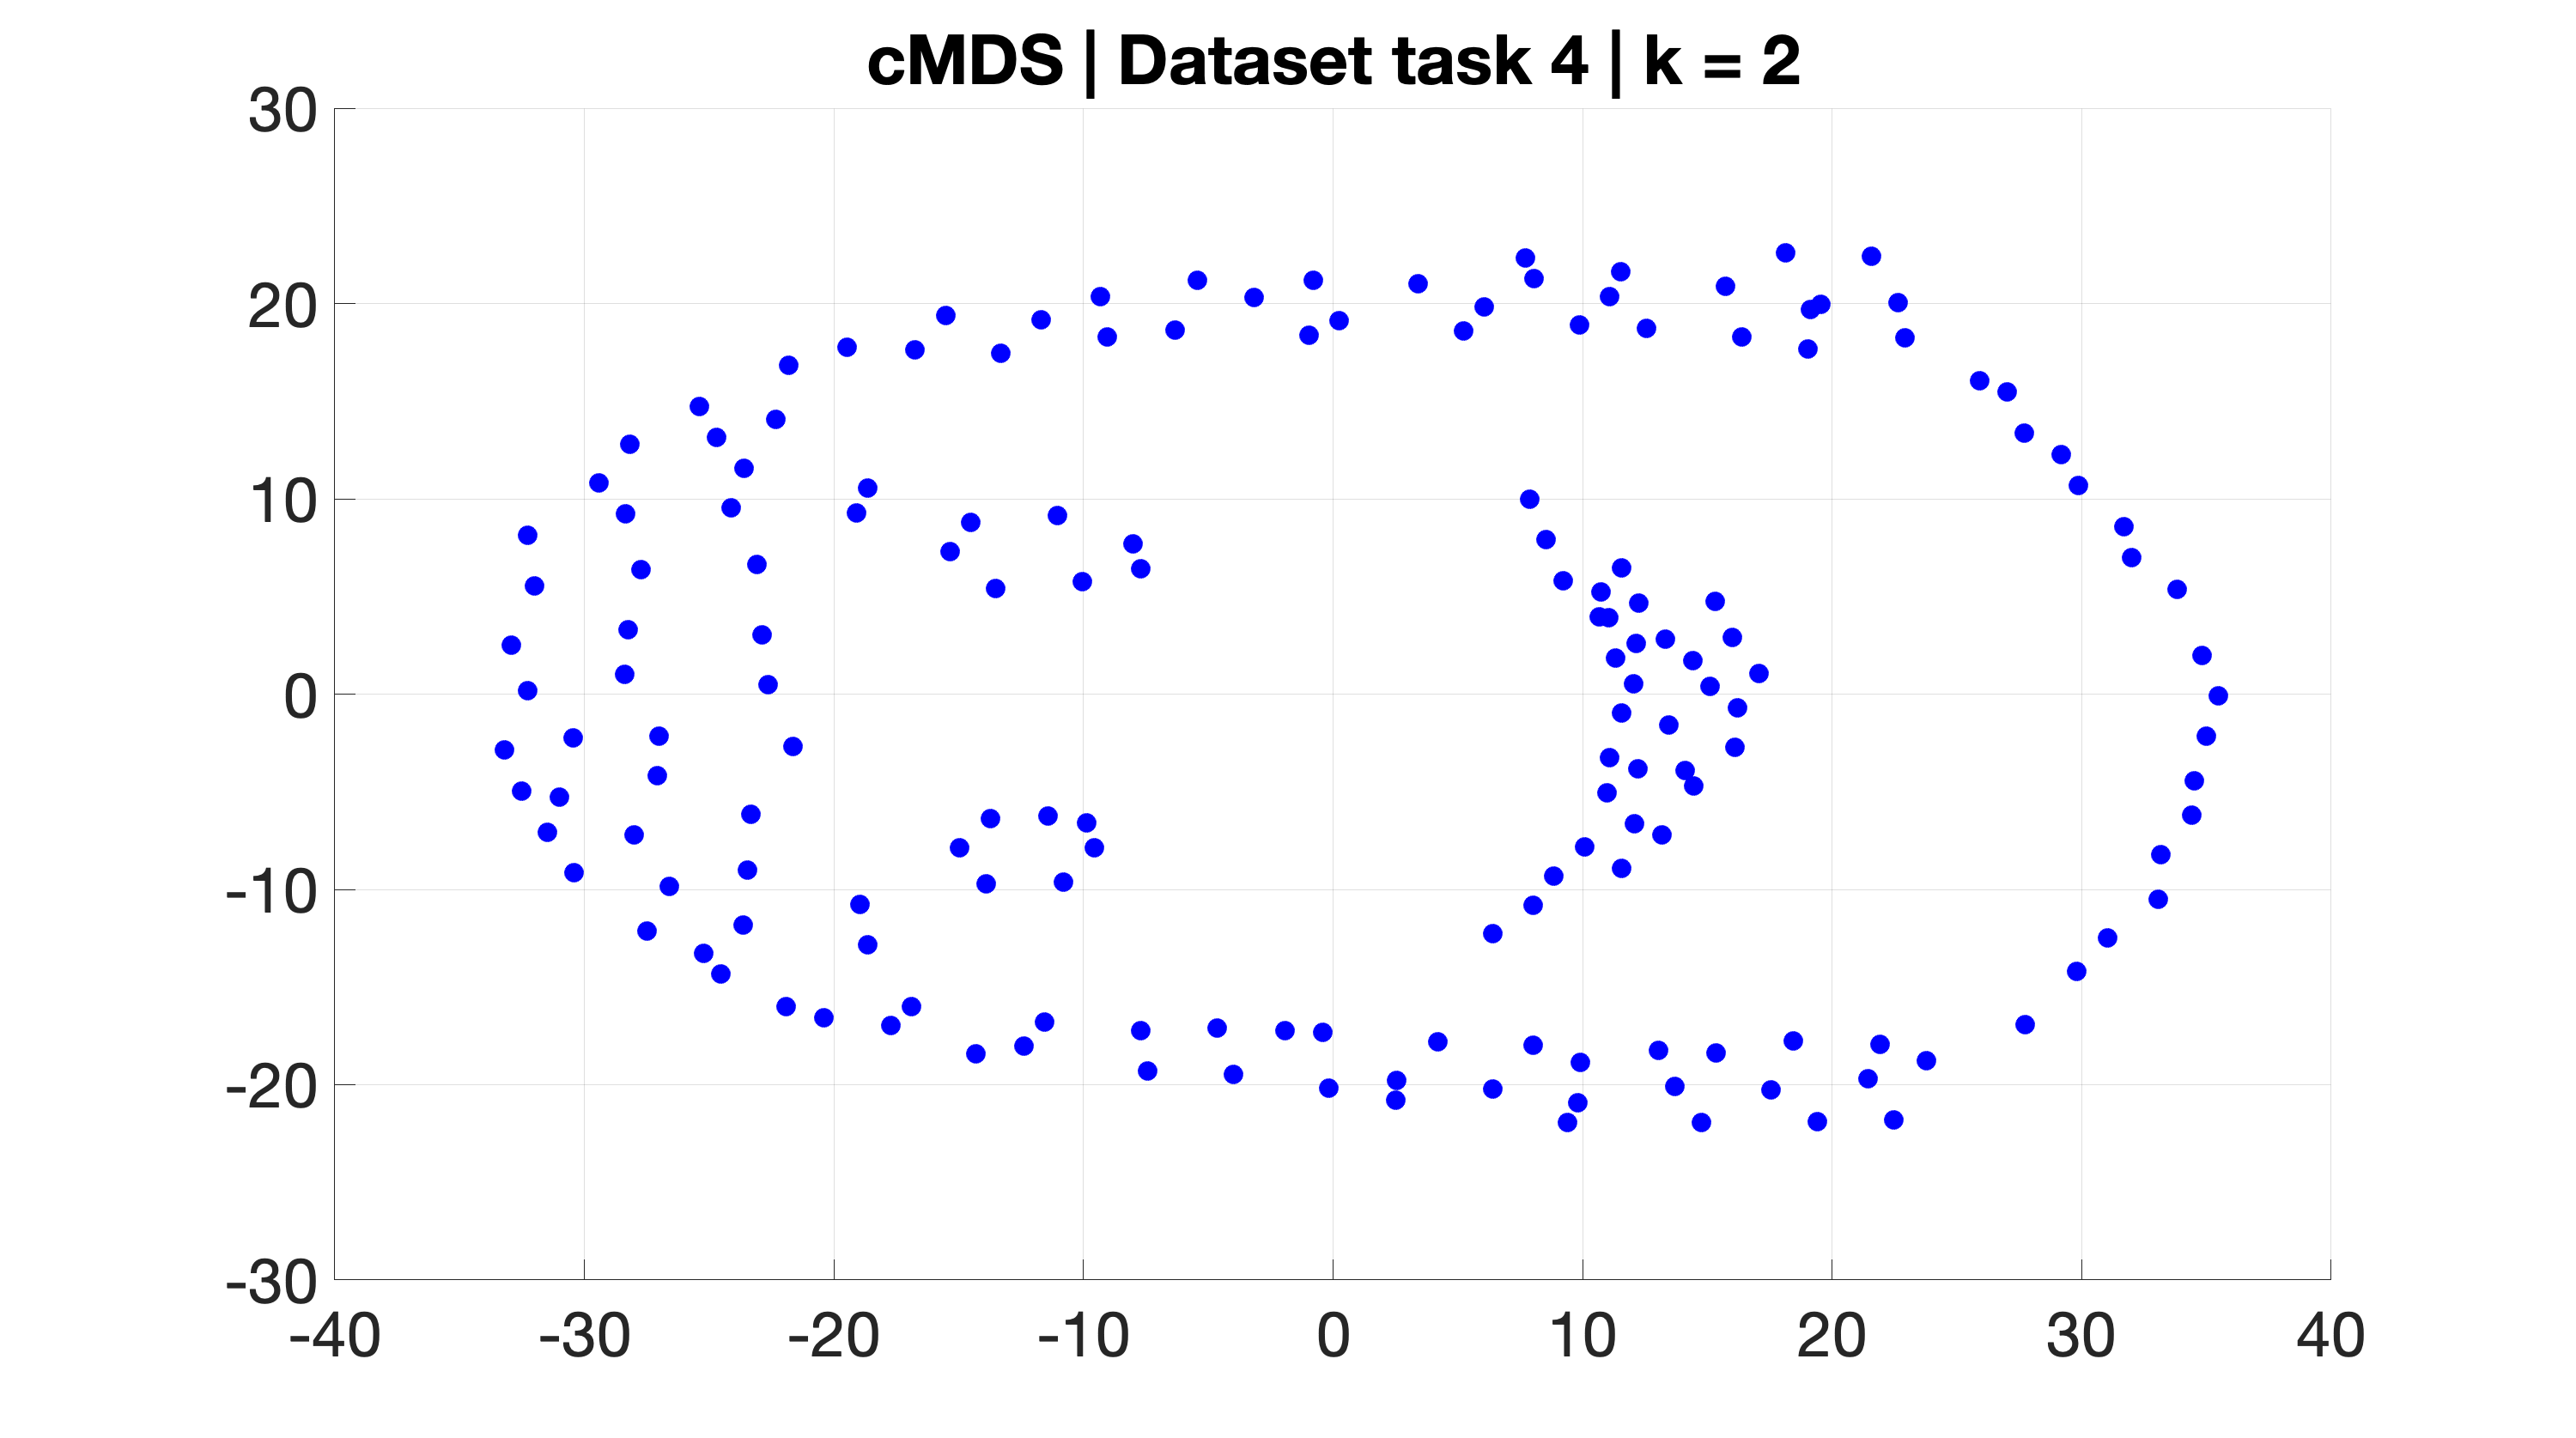
\includegraphics[width=0.9\textwidth]{figures/task4_extra_sol.png}
			\label{fig:task4_LM}
		\caption{Solução método cMDS.}
	\end{figure}
	\begin{itemize}
		\item A solução corresponde a uma translação e rotação das duas soluções anteriores.
	\end{itemize}
\end{frame}

\begin{comment}
\begin{frame}{Part 3 - Task 4 - cMDS}
\begin{itemize}
\item A solução corresponde a uma translação e rotação das duas soluções anteriores.
\item Mais eficiente do que LM.
\item É evidente a existência de graus de liberdade de rotação e translação.
\end{itemize}
\end{frame}
\end{comment}



%\begin{frame}{Slide with bullet points}
%	This is a bullet list of two points:
%    \begin{itemize}
%		\item Point one
%        \item Point two
%	\end{itemize}
%\end{frame}
%
%\begin{frame}{Slide with two columns}
%	\begin{columns}
%		\column{.5\textwidth}
%        Text goes in first column.
%        
%        \column{.5\textwidth}
%        Text goes in second column
%	\end{columns}
%\end{frame}
%
%\section{Section Two}
%
%\begin{frame}{Slide with table}
%	\input{tables/table1.tex}
%\end{frame}
%
%\begin{frame}{Slide with figure}
%	\begin{figure}[H]
%		\centering
%        \includegraphics[width=.5\textwidth]{figures/figure1.png}
%        \caption{Caption for figure one.}
%        \label{fig:figure1}
%	\end{figure}
%\end{frame}
%
%\begin{frame}{Slide with references}
%	This is to reference a figure (Figure \ref{fig:figure1})\\
%    This it to reference a table (Table \ref{tab:table1})\\
%    This is to cite an article \cite{Ahmed2018a}\\
%    This is to add an article to the references without mentioning in the text \nocite{Ahmed2018a}\\
%\end{frame}
%\section{References}
%
%% Adding the option 'allowframebreaks' allows the contents of the slide to be expanded in more than one slide.
%\begin{frame}[allowframebreaks]{References}
%	\tiny\bibliography{references}
%	\bibliographystyle{apalike}
%\end{frame}

\end{document}
